%%%%%%%%%%%%%%%%%%%%%%%%%%%%%%%%%%%%%%%%%%%%%%%%%%%%%%%%%%%%%%%%%%%%%%%%%%%%%%%
%%%%%%%%%%%%%%%%%%%%%%%%%%%%%%%%%%%%%%%%%%%%%%%%%%%%%%%%%%%%%%%%%%%%%%%%%%%%%%%
%%%%  APPENDIX B
%%%%%%%%%%%%%%%%%%%%%%%%%%%%%%%%%%%%%%%%%%%%%%%%%%%%%%%%%%%%%%%%%%%%%%%%%%%%%%%
%%%%%%%%%%%%%%%%%%%%%%%%%%%%%%%%%%%%%%%%%%%%%%%%%%%%%%%%%%%%%%%%%%%%%%%%%%%%%%%

\chapter{Numerical calculations for the Hubbard Hamiltonian in the compensated
lattice}
\label{app:numerical}


In this appendix we present the results of numerical calculations for a
homogeneous Hubbard model in a simple cubic lattice, which serve as the basis
for our implementation of the local density approximation (LDA).  As we
mentioned in Chapter~\ref{chap:hubbardmodel}, our theory collaborators provide
us with results of DQMC and NLCE calculations in a grid of $U/t$, $T/t$, and
$\mu/t$ values.    

The DQMC and NLCE results complement each other.  DQMC can provide results at
arbitrary chemical potential down to the N\'{e}el transition temperature if the
coupling is weak, $U/t\leq 9$.   For strong coupling, DQMC runs into the sign
problem, but NLCE can provide results for arbitrary $U/t$ down to $T=0.4t$.
For this reason we turn to NLCE results for for large values of $U/t$. 

In the sections below, we present the complete NLCE and DQMC data sets and
explain how we use the available data to interpolate and obtain the values of
the thermodynamic quantities for arbitrary values of $U/t$, $T/t$ and $\mu/t$. 

The full data set, along with more plots and the code used for interpolation
are available online at ~\cite{PedroMDuarte:12780}. 
 

\section{NLCE} 
 
The NLCE data set was provided by E. Khatami.   It includes exact results down
to $T/t=1.6$ for a wide range of $\mu/T$, for the following thermodynamic
quantities (all quantities are given per lattice site):

\begin{multicols}{2}
\begin{itemize}
  \item energy 
  \item energy fluctuations
  \item density
  \item density fluctuations 
  \item $S_{z}$ fluctuations
  \item entropy
  \item specific heat
  \item double occupancy
  \item nearest neighbor spin correlations
  \item spin structure for $\bv{Q}=\bv{\pi}$
  \item spin structure for $\bv{Q}=\bv{\theta}$
\end{itemize}
\end{multicols}

\vspace{-1em}
For temperatures below $T/t=1.6$,  an Euler resummation is
performed~\cite{Tang2013} to obtain estimates of the thermodynamic quantities.
At values of the temperature around $T/t=0.4$ the results start getting very
noisy, however, we can extract a usable data set by applying a low pass filter
to the data\footnote{The type of filter used is the Savitzky-Golay filter
\url{http://www.wire.tu-bs.de/OLDWEB/mameyer/cmr/savgol.pdf}}.  The original
data and the filtered data are shown in Fig.~\ref{fig:NLCE_T0.40} for the
density, entropy and $s_{\bv{\pi}}$ at a the lowest temperature $T/t=0.4$.  For
larger values of $T/t$ the data is not as noisy, as shown for the density in
Fig.~\ref{fig:NLCE_Thigher}.  We still use the filter up to $T/t=1.4$ to remove
some spurious points that show up in the data.  At $T/t > 1.6$ the data is
exact and it has no spurious points.

\begin{figure}
    \centering
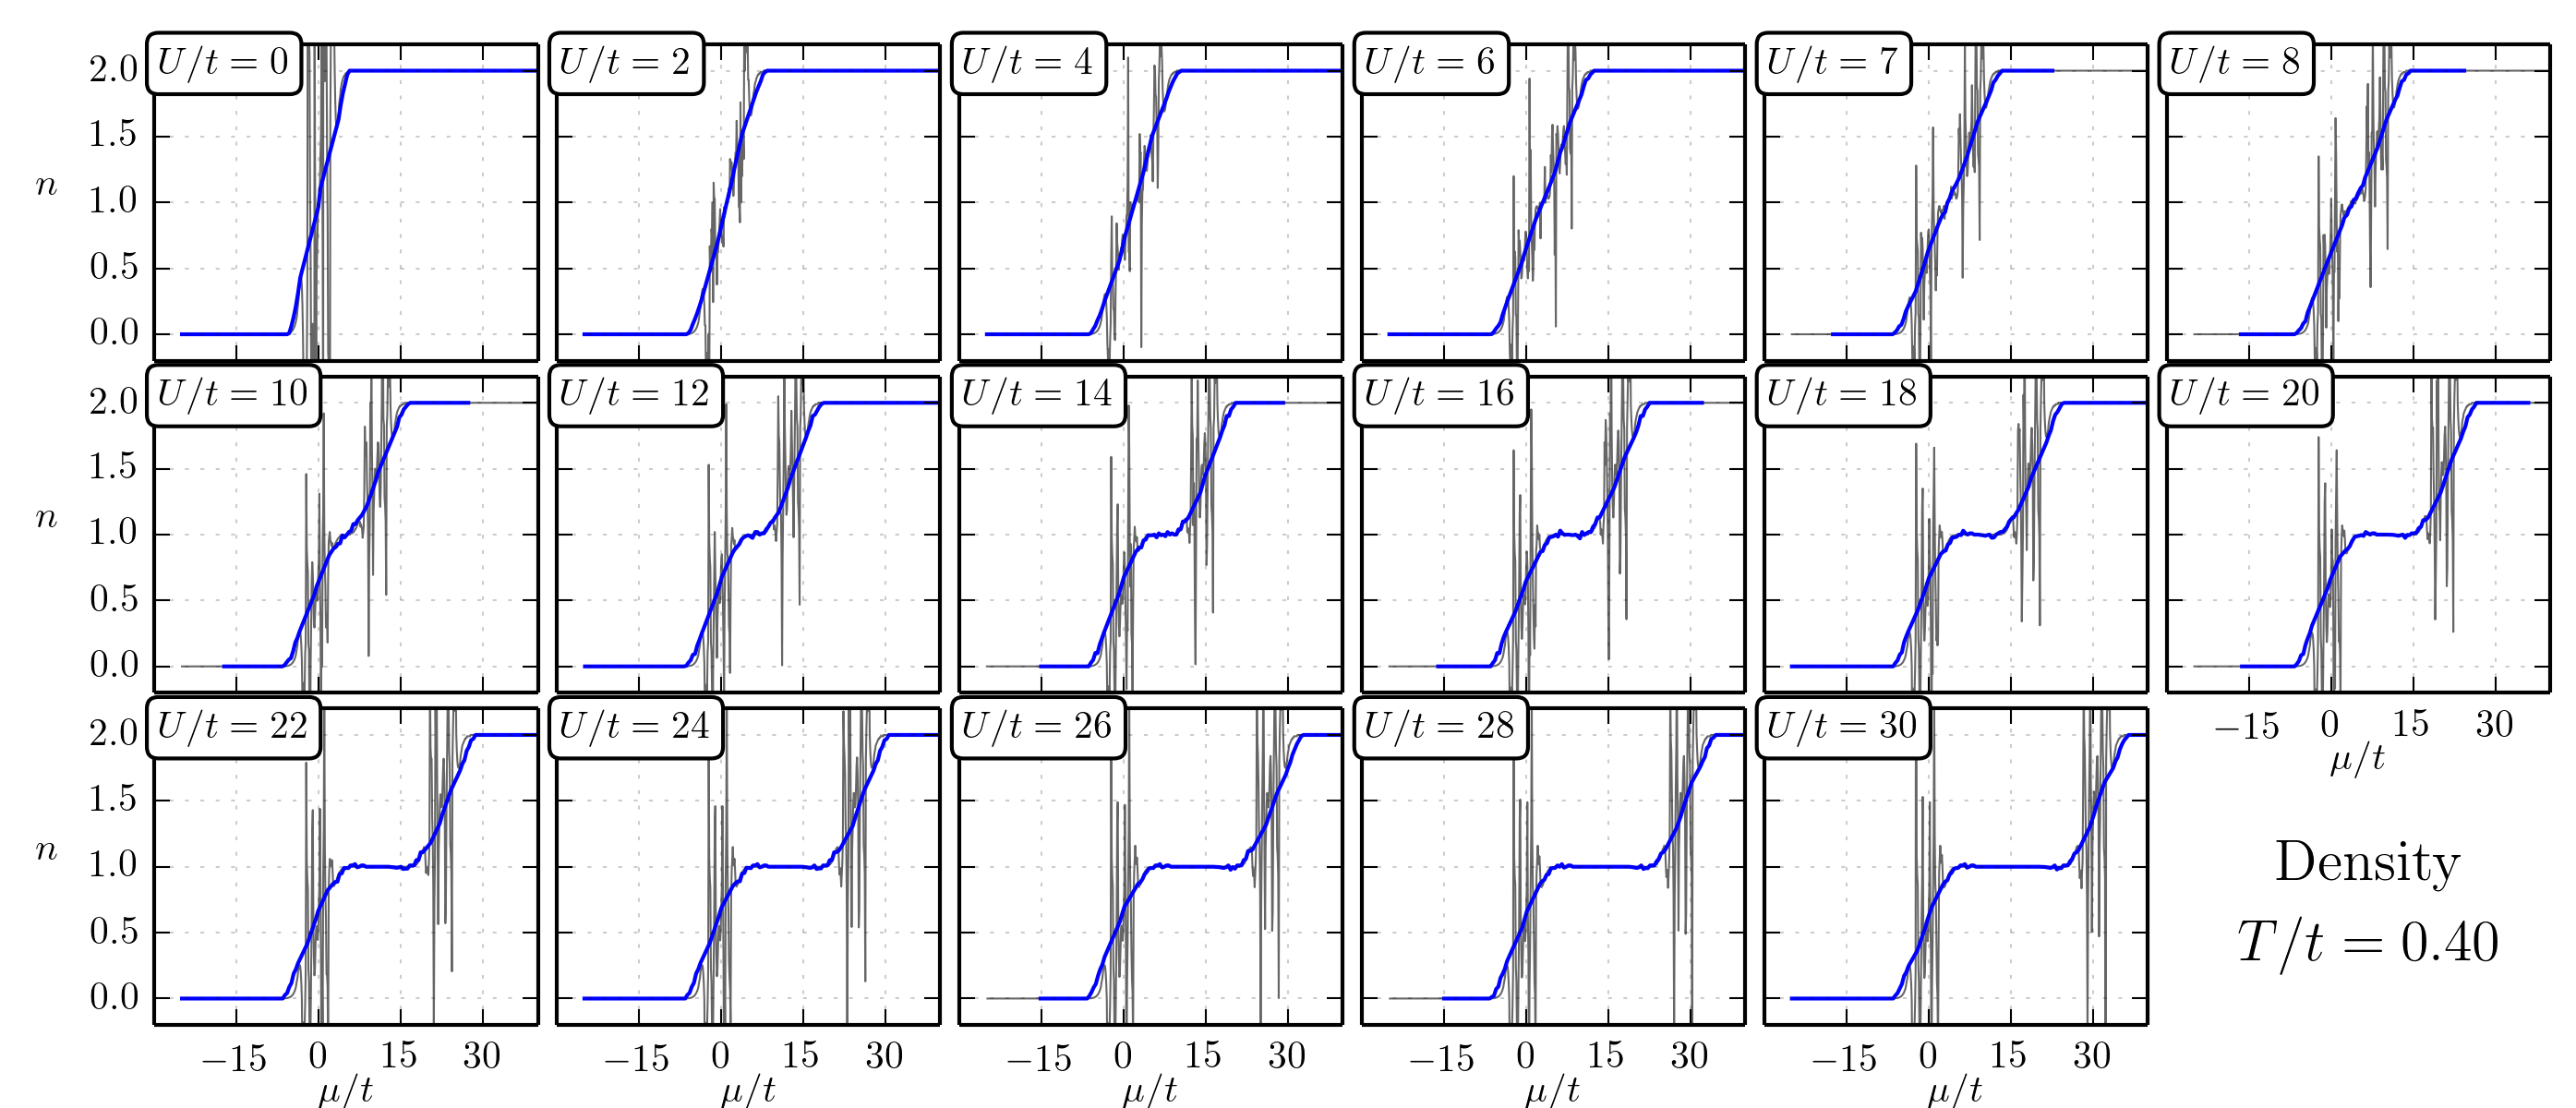
\includegraphics[width=1.0\textwidth]{../figures/hubbard-data/dataplots/NLCE8_Final/density/T0_40.png}
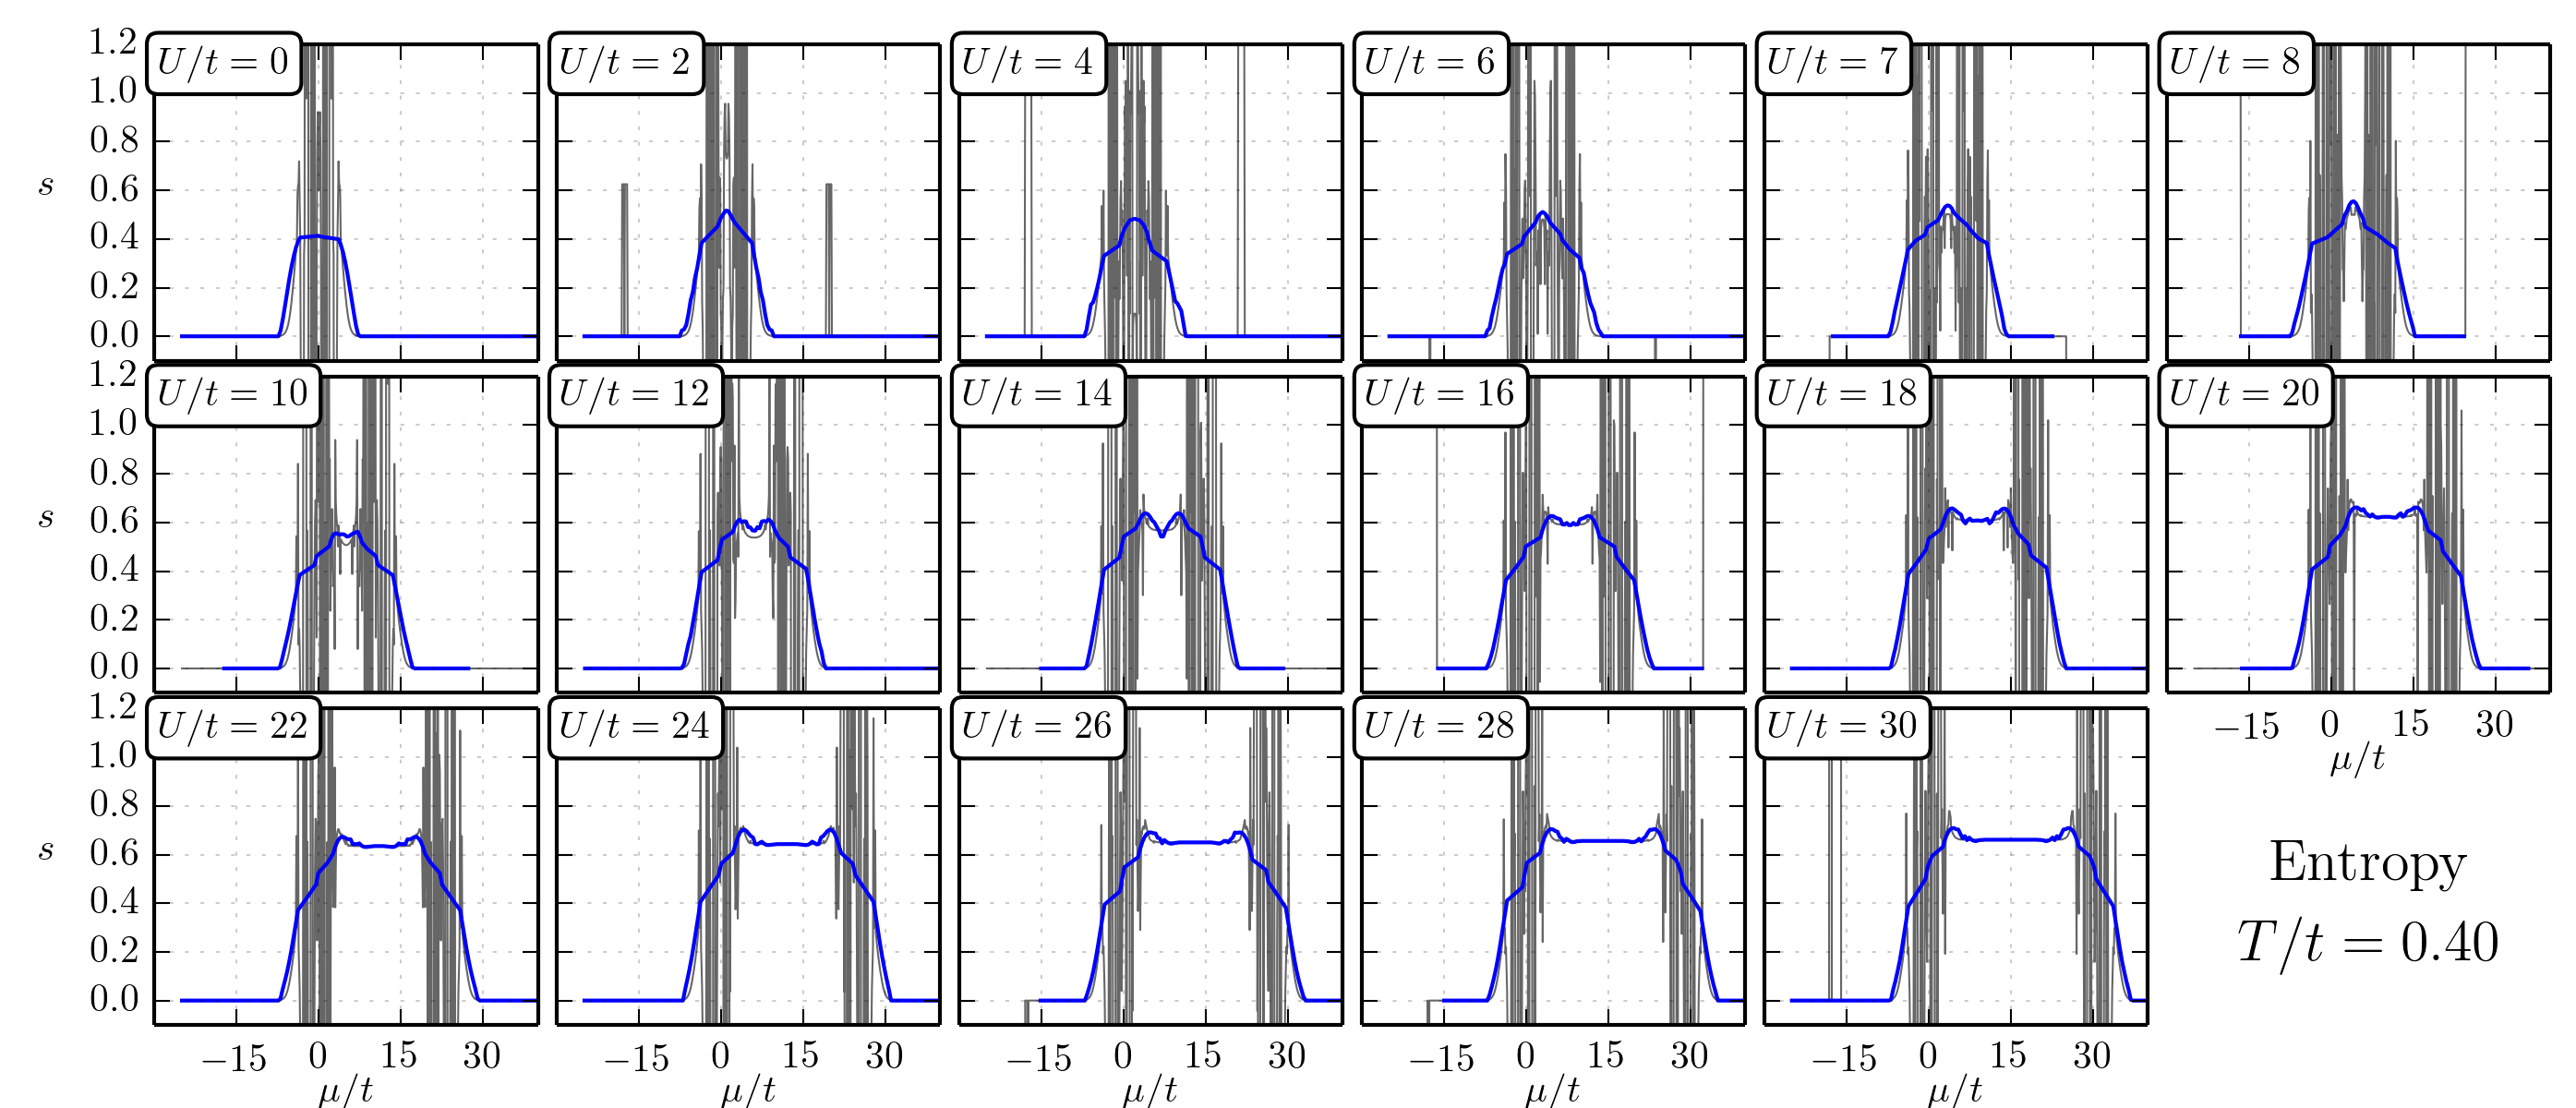
\includegraphics[width=1.0\textwidth]{../figures/hubbard-data/dataplots/NLCE8_Final/entropy/T0_40.png}
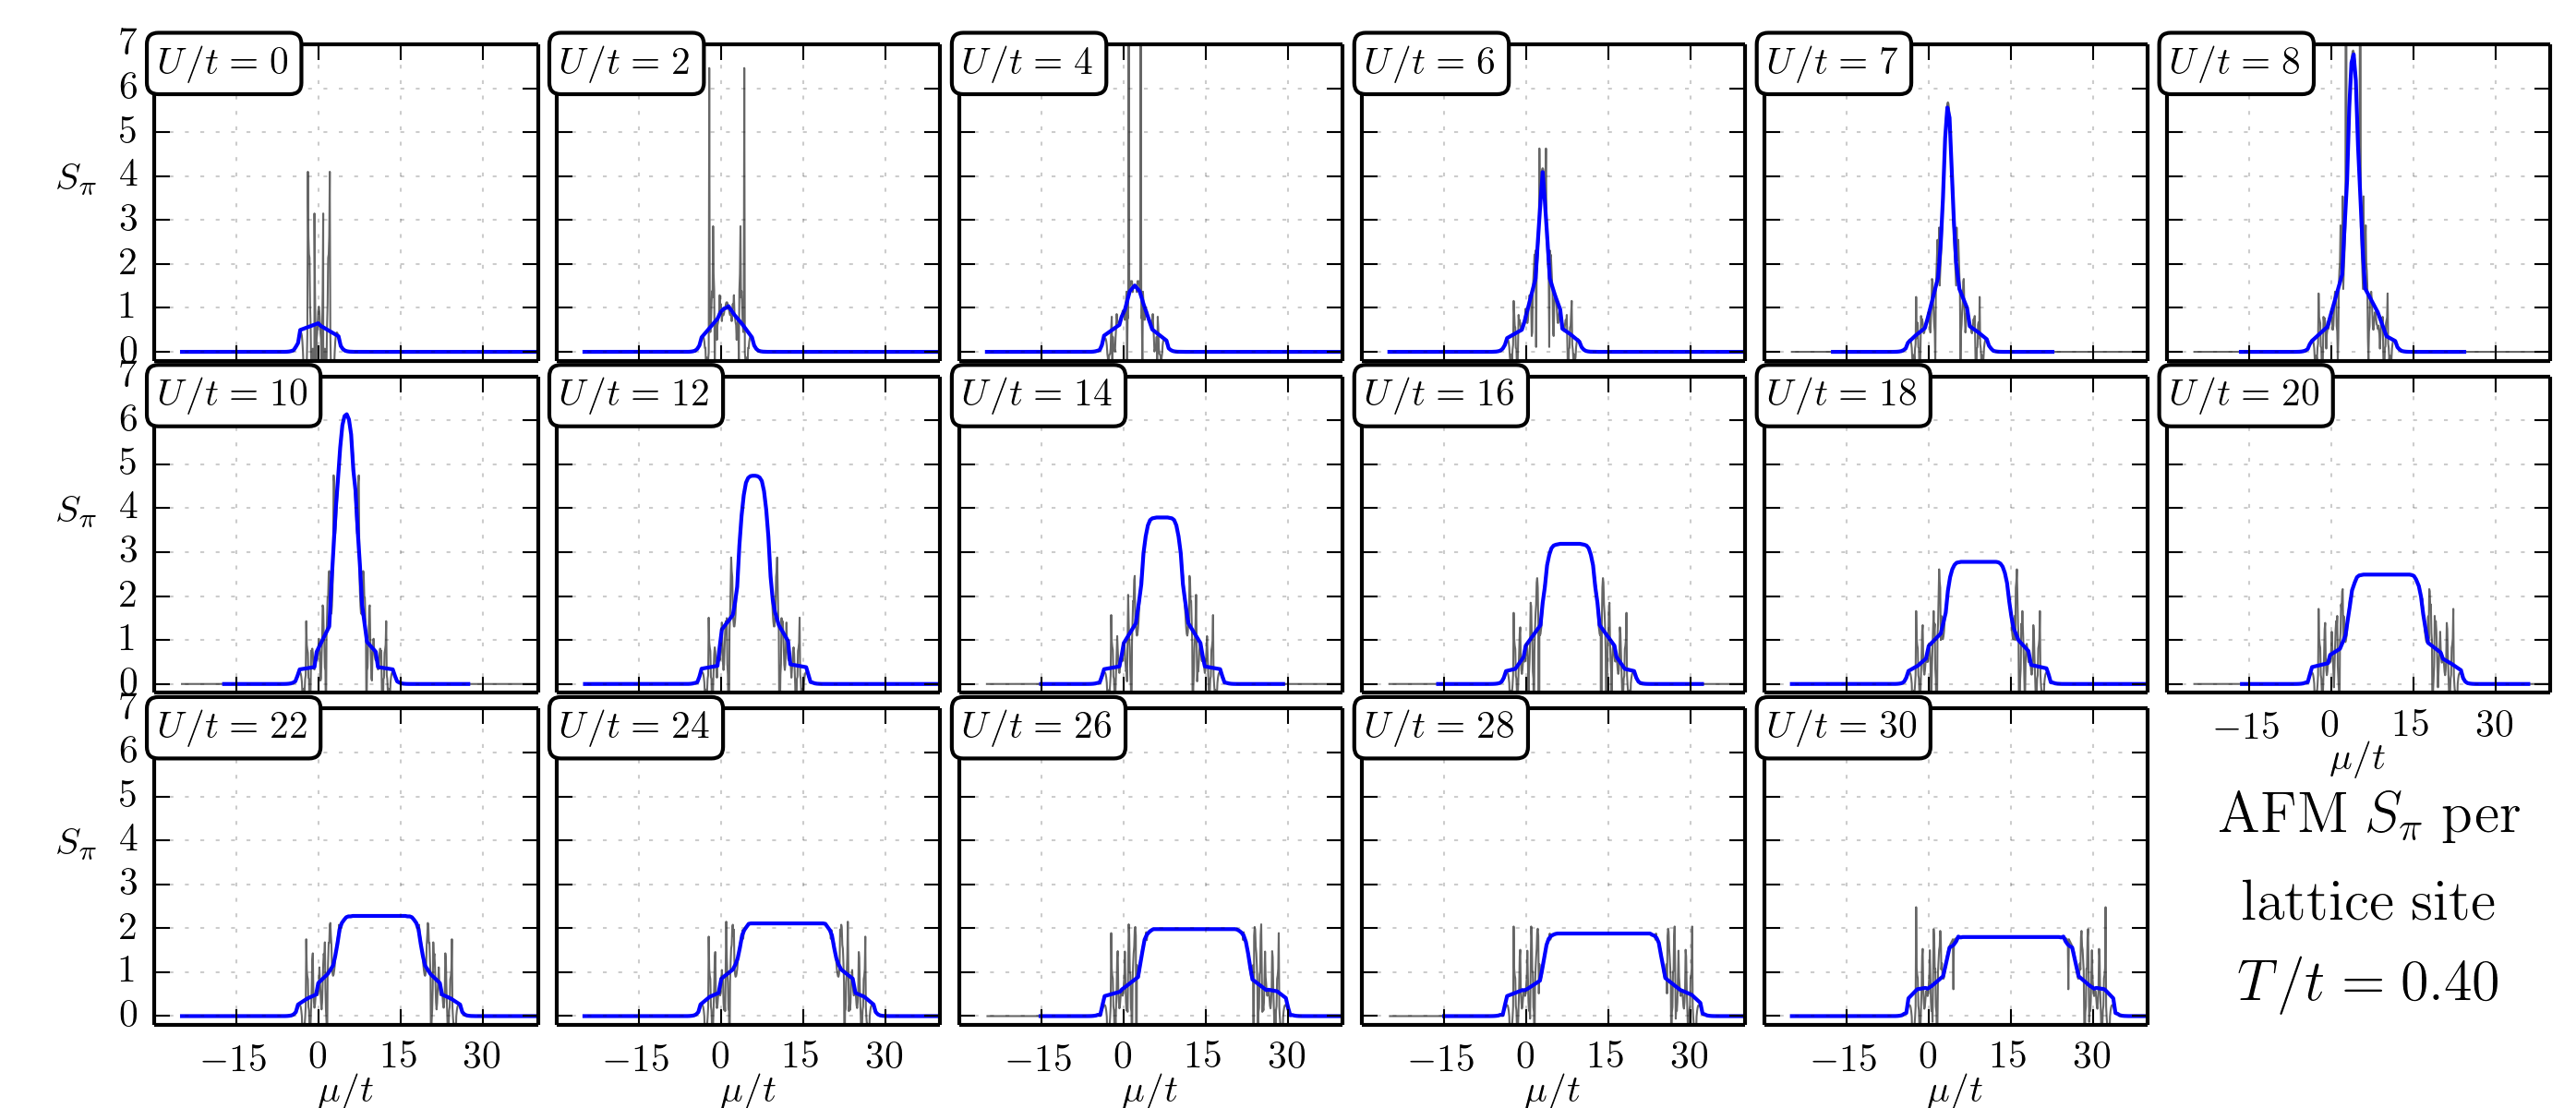
\includegraphics[width=1.0\textwidth]{../figures/hubbard-data/dataplots/NLCE8_Final/spi/T0_40.png}
\caption{Lowest temperature data accessible to the NLCE by extrapolation,
$T/t=0.4$.  The original data provided by Ehsan is shown in gray and the data
after filtering is shown in blue.}
\label{fig:NLCE_T0.40}
\end{figure}

\begin{figure}
    \centering
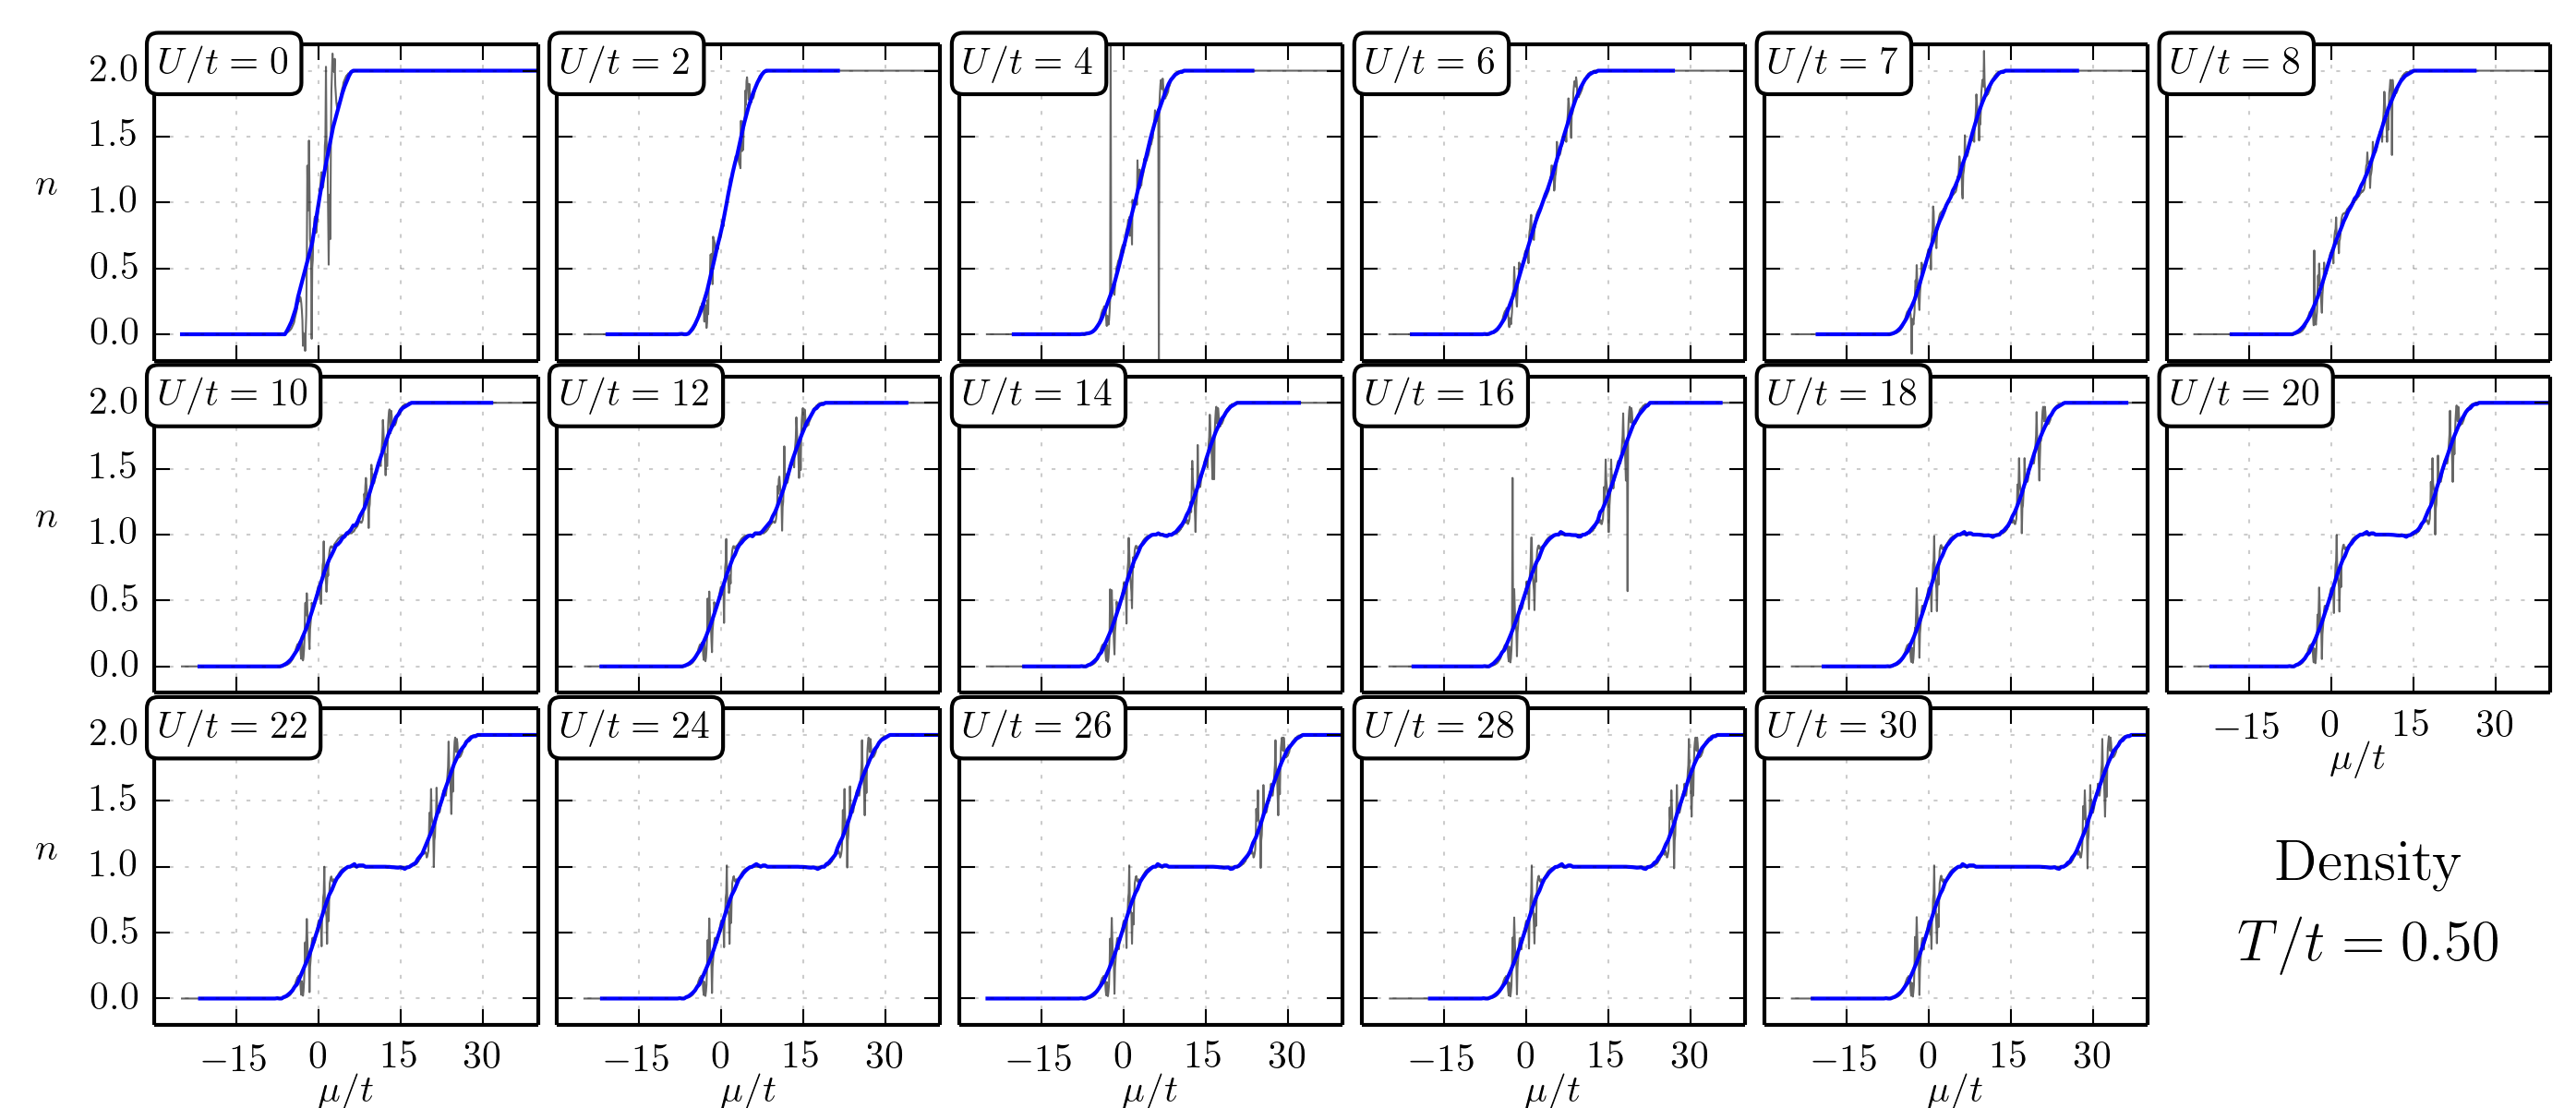
\includegraphics[width=1.0\textwidth]{../figures/hubbard-data/dataplots/NLCE8_Final/density/T0_50.png}
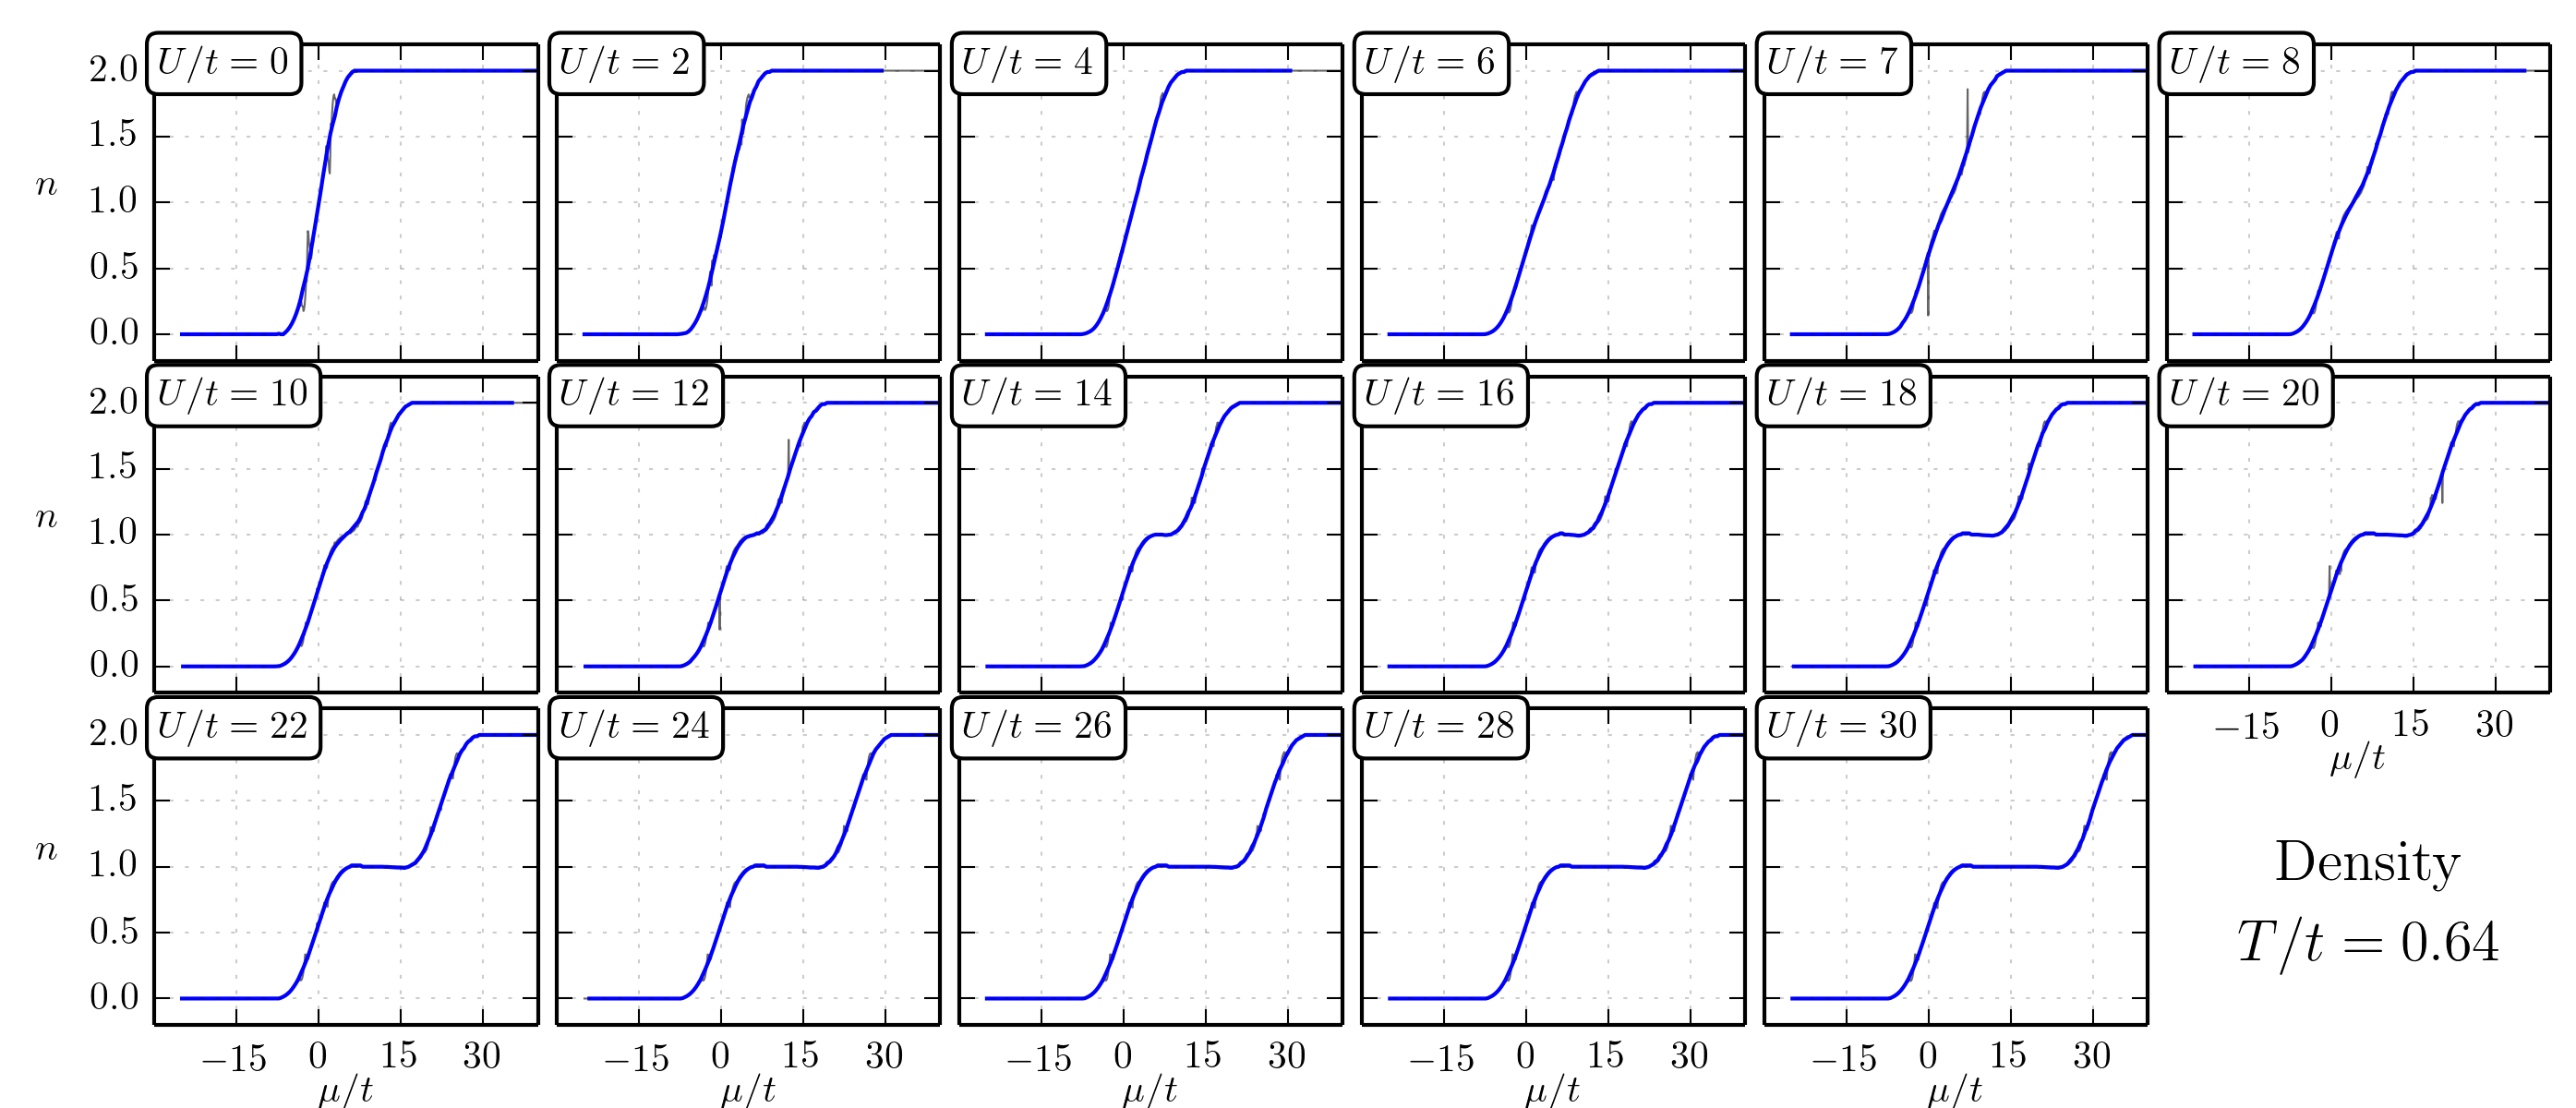
\includegraphics[width=1.0\textwidth]{../figures/hubbard-data/dataplots/NLCE8_Final/density/T0_64.png}
\caption{Larger values of $T$ do not show as much noise as $T/t=0.4$.}
\label{fig:NLCE_Thigher}
\end{figure}


The most important quantity for comparing to our results is the spin structure
factor for $\bv{Q}=\bv{\pi}$.   The data for the spin structure factor per
lattice site, $s_{\bv{\pi}}/n$ provided by NLCE for some values of $U/t$ is
shown in Fig.~\ref{fig:NLCESpin}.  

\begin{figure}
    \centering
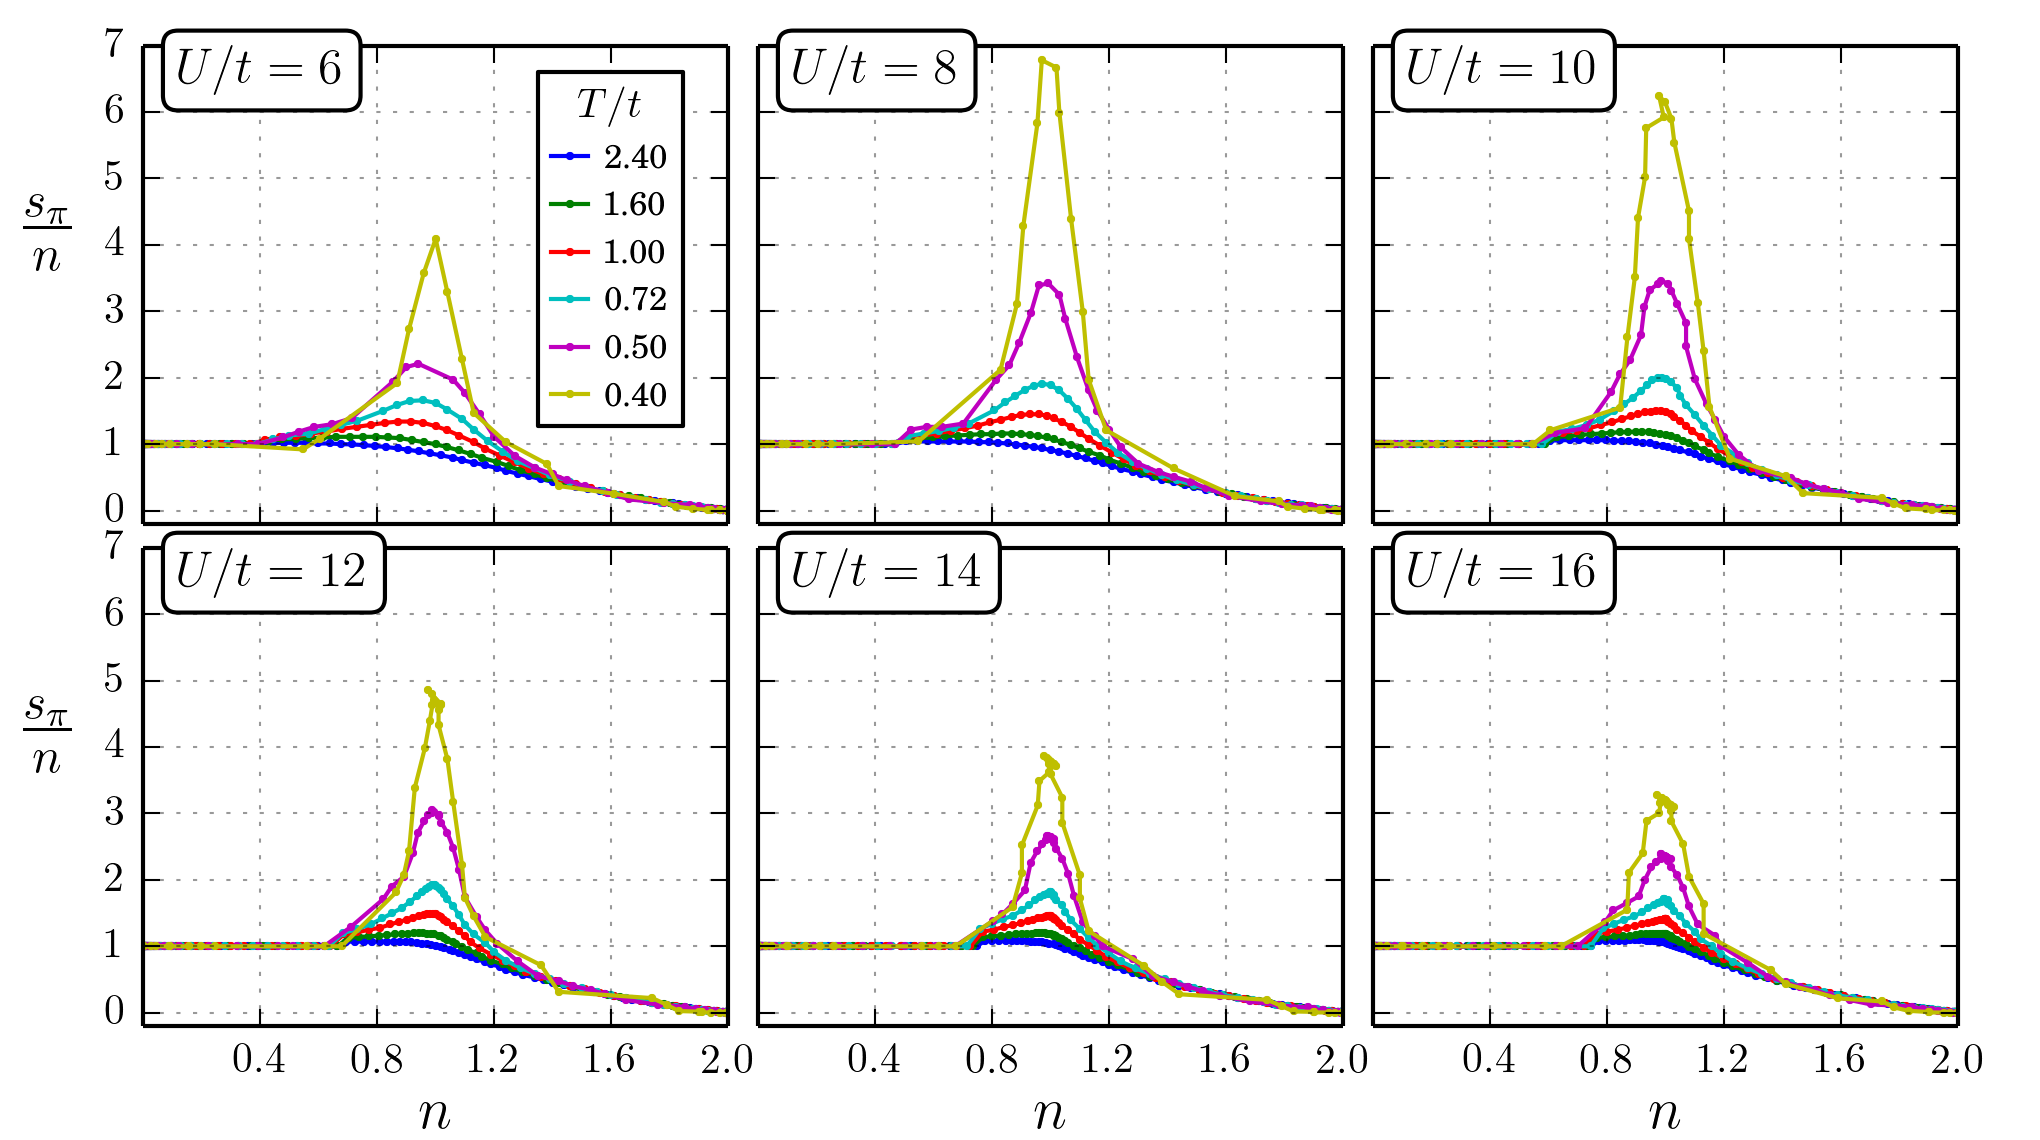
\includegraphics[width=\textwidth]{../figures/hubbard-data/dataplots/NLCE8_Final/Spi_varyU_varyT.png}
\caption{NLCE $S_{\pi}/n$  data for various interactions and temperatures.  }
\label{fig:NLCESpin}
\end{figure}


\section{ DQMC data } 

The DQMC data set was provided by T. Paiva.  It includes results for the
following thermodynamic quantities:

\begin{multicols}{2}
\begin{itemize}
  \item density
  \item entropy
  \item double occupancy
  \item spin structure for $\bv{Q}=\bv{\pi}$
  \item spin structure for $\bv{Q}=\bv{\theta}$
\end{itemize}
\end{multicols}

The DQMC data does not suffer from significant noise problems for small values
of $T/t$, however due to the sign problem it can only reach low temperatures
for $U/t\leq10$.  In Figs.~\ref{fig:QMCdens} to ~\ref{fig:QMCsth} we show the
available DQMC data for density, entropy and the spin structure factor per
particle for $\bv{Q}=\bv{\pi}$ and $\bv{Q}=\bv{\theta}$.

\begin{figure}
    \centering
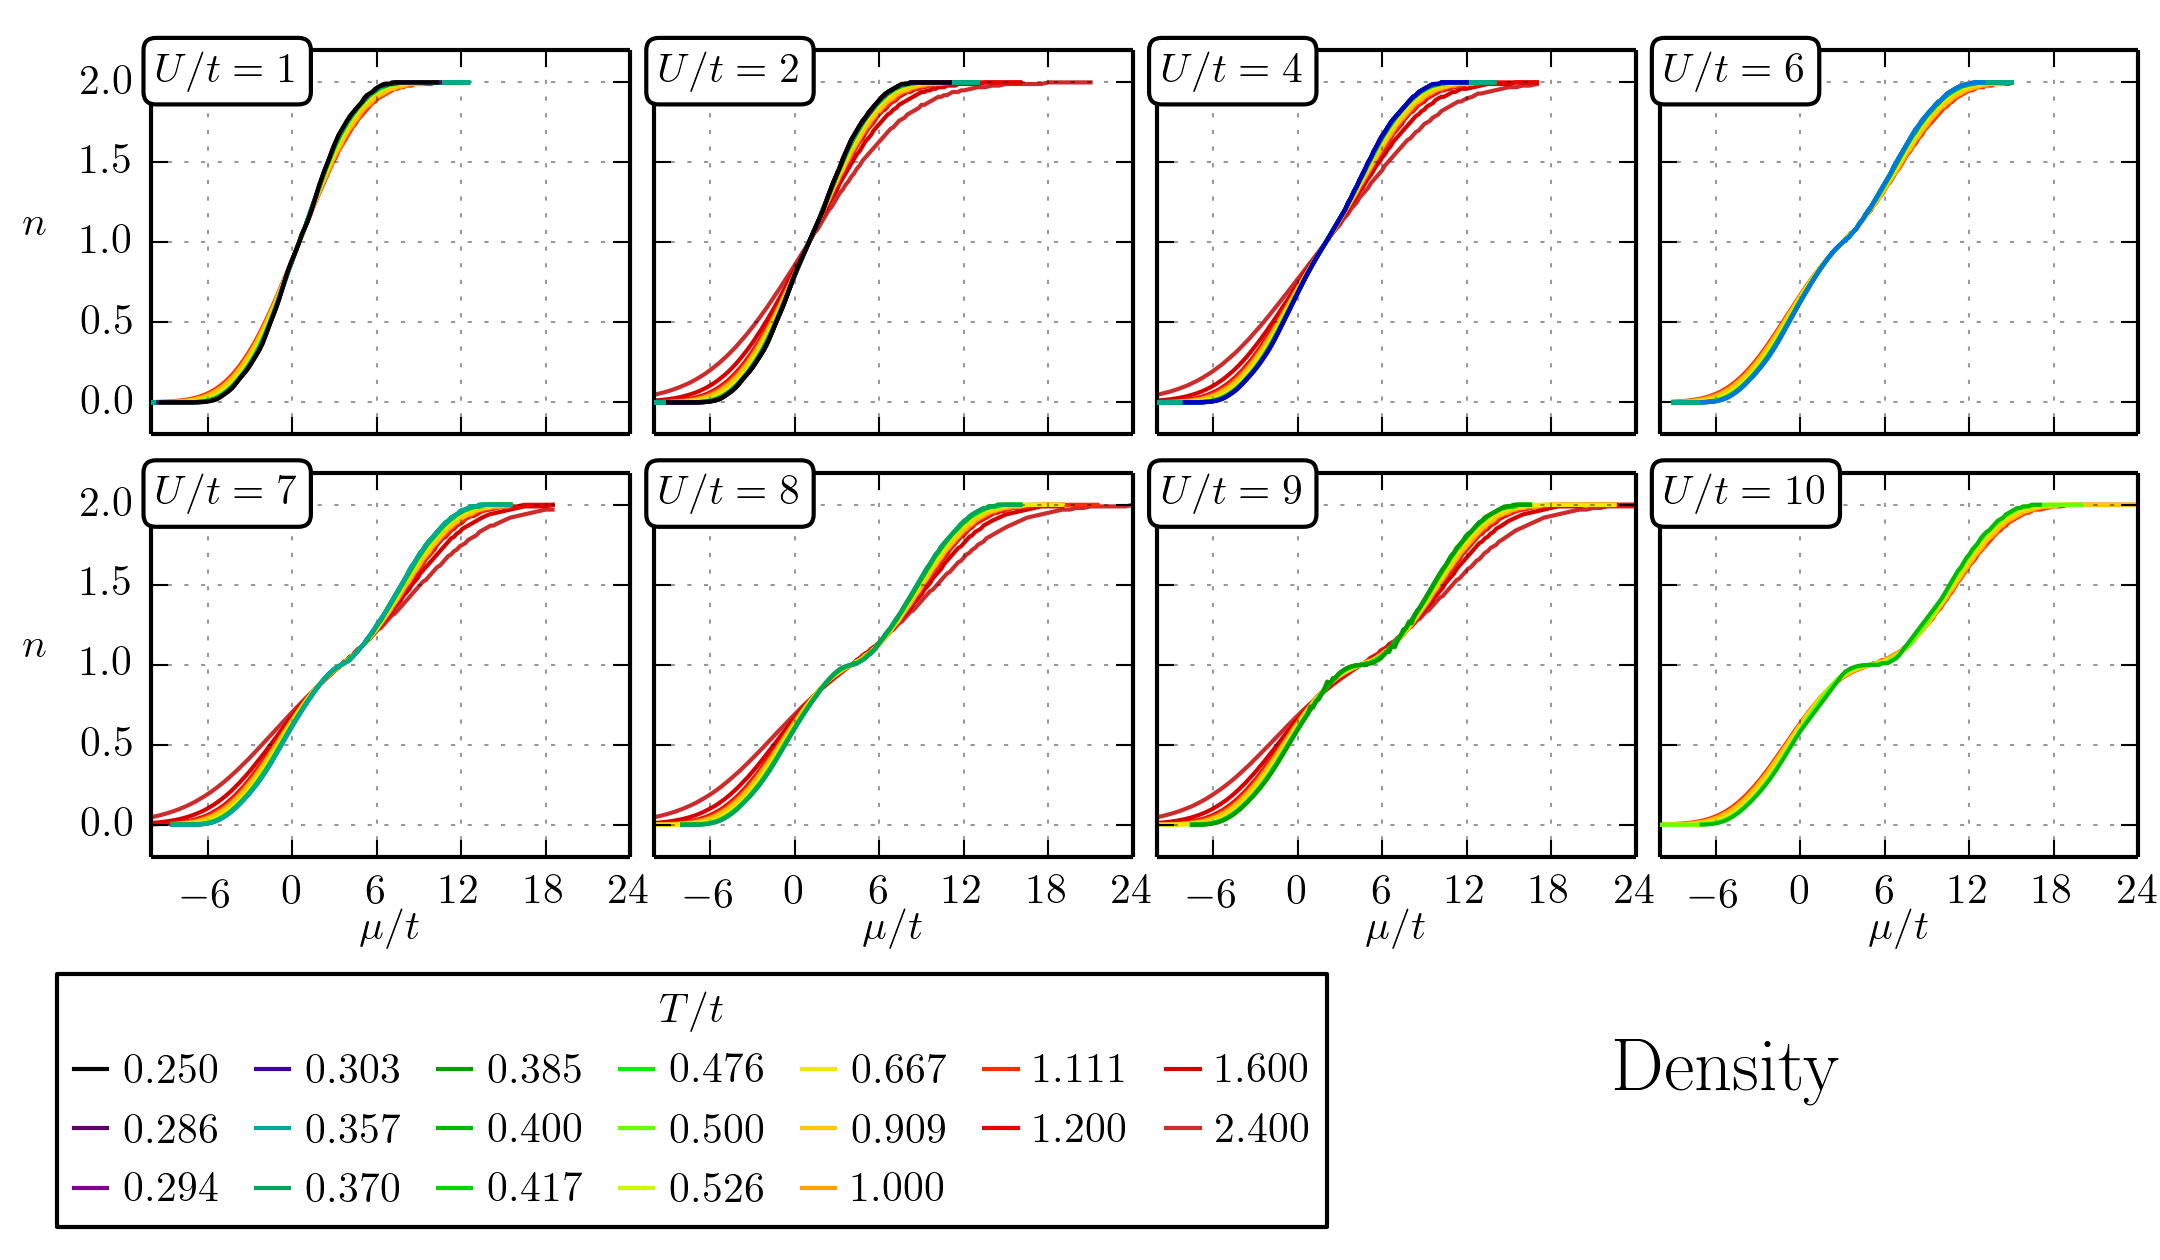
\includegraphics[width=1.0\textwidth]{../figures/hubbard-data/dataplots/QMC_Final/density_10.png}
\caption{ DQMC results for the density. } 
\label{fig:QMCdens}
\end{figure}
\begin{figure}
    \centering
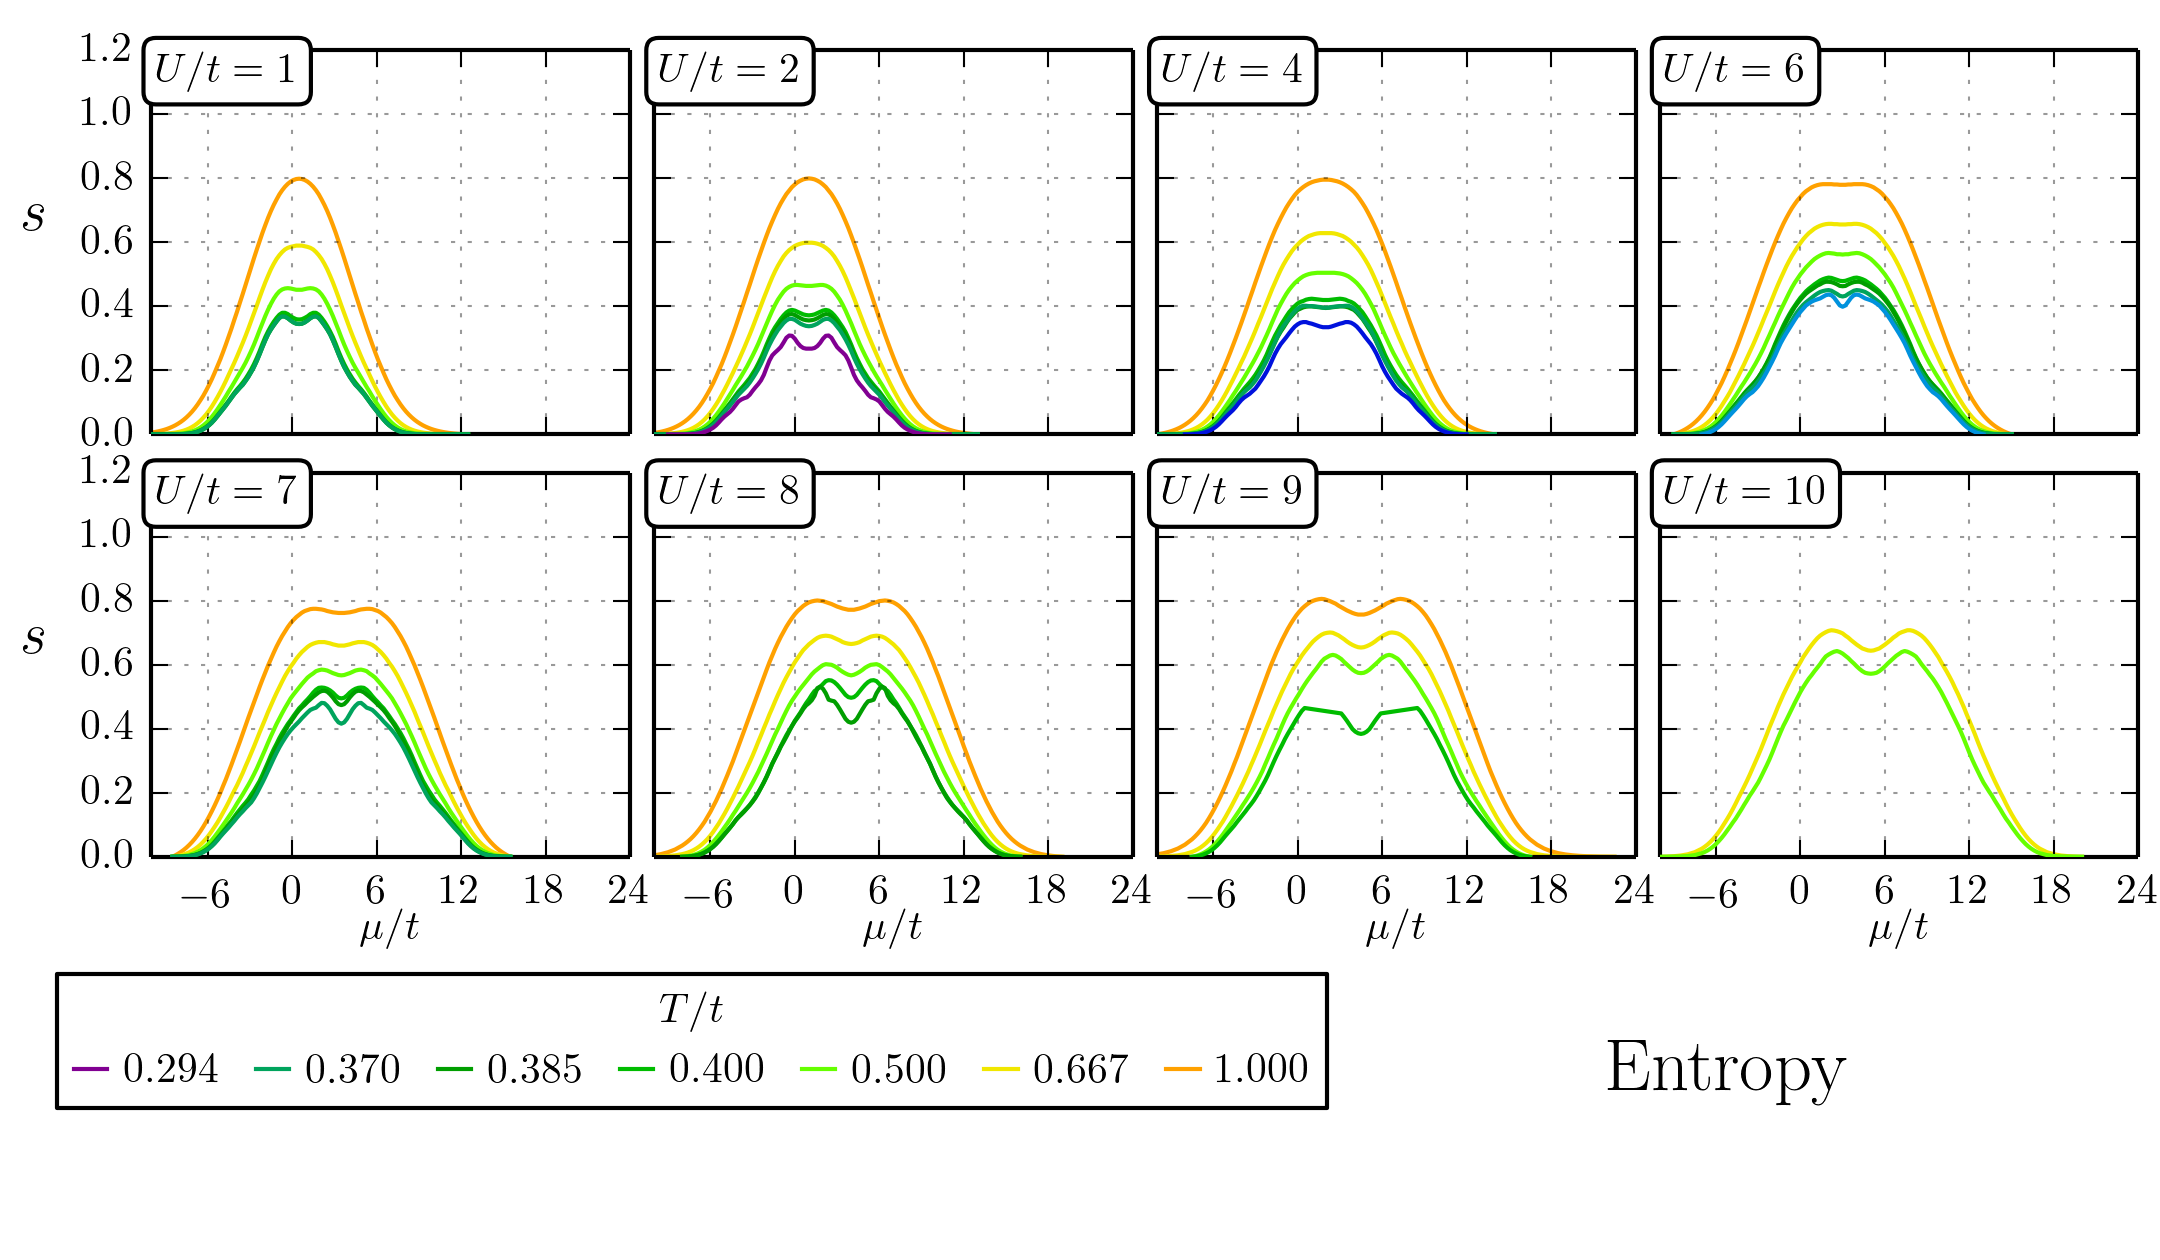
\includegraphics[width=1.0\textwidth]{../figures/hubbard-data/dataplots/QMC_Final/entropy_10.png}
\caption{ DQMC results for the entropy. } 
\label{fig:QMCent}
\end{figure}
\begin{figure}
    \centering
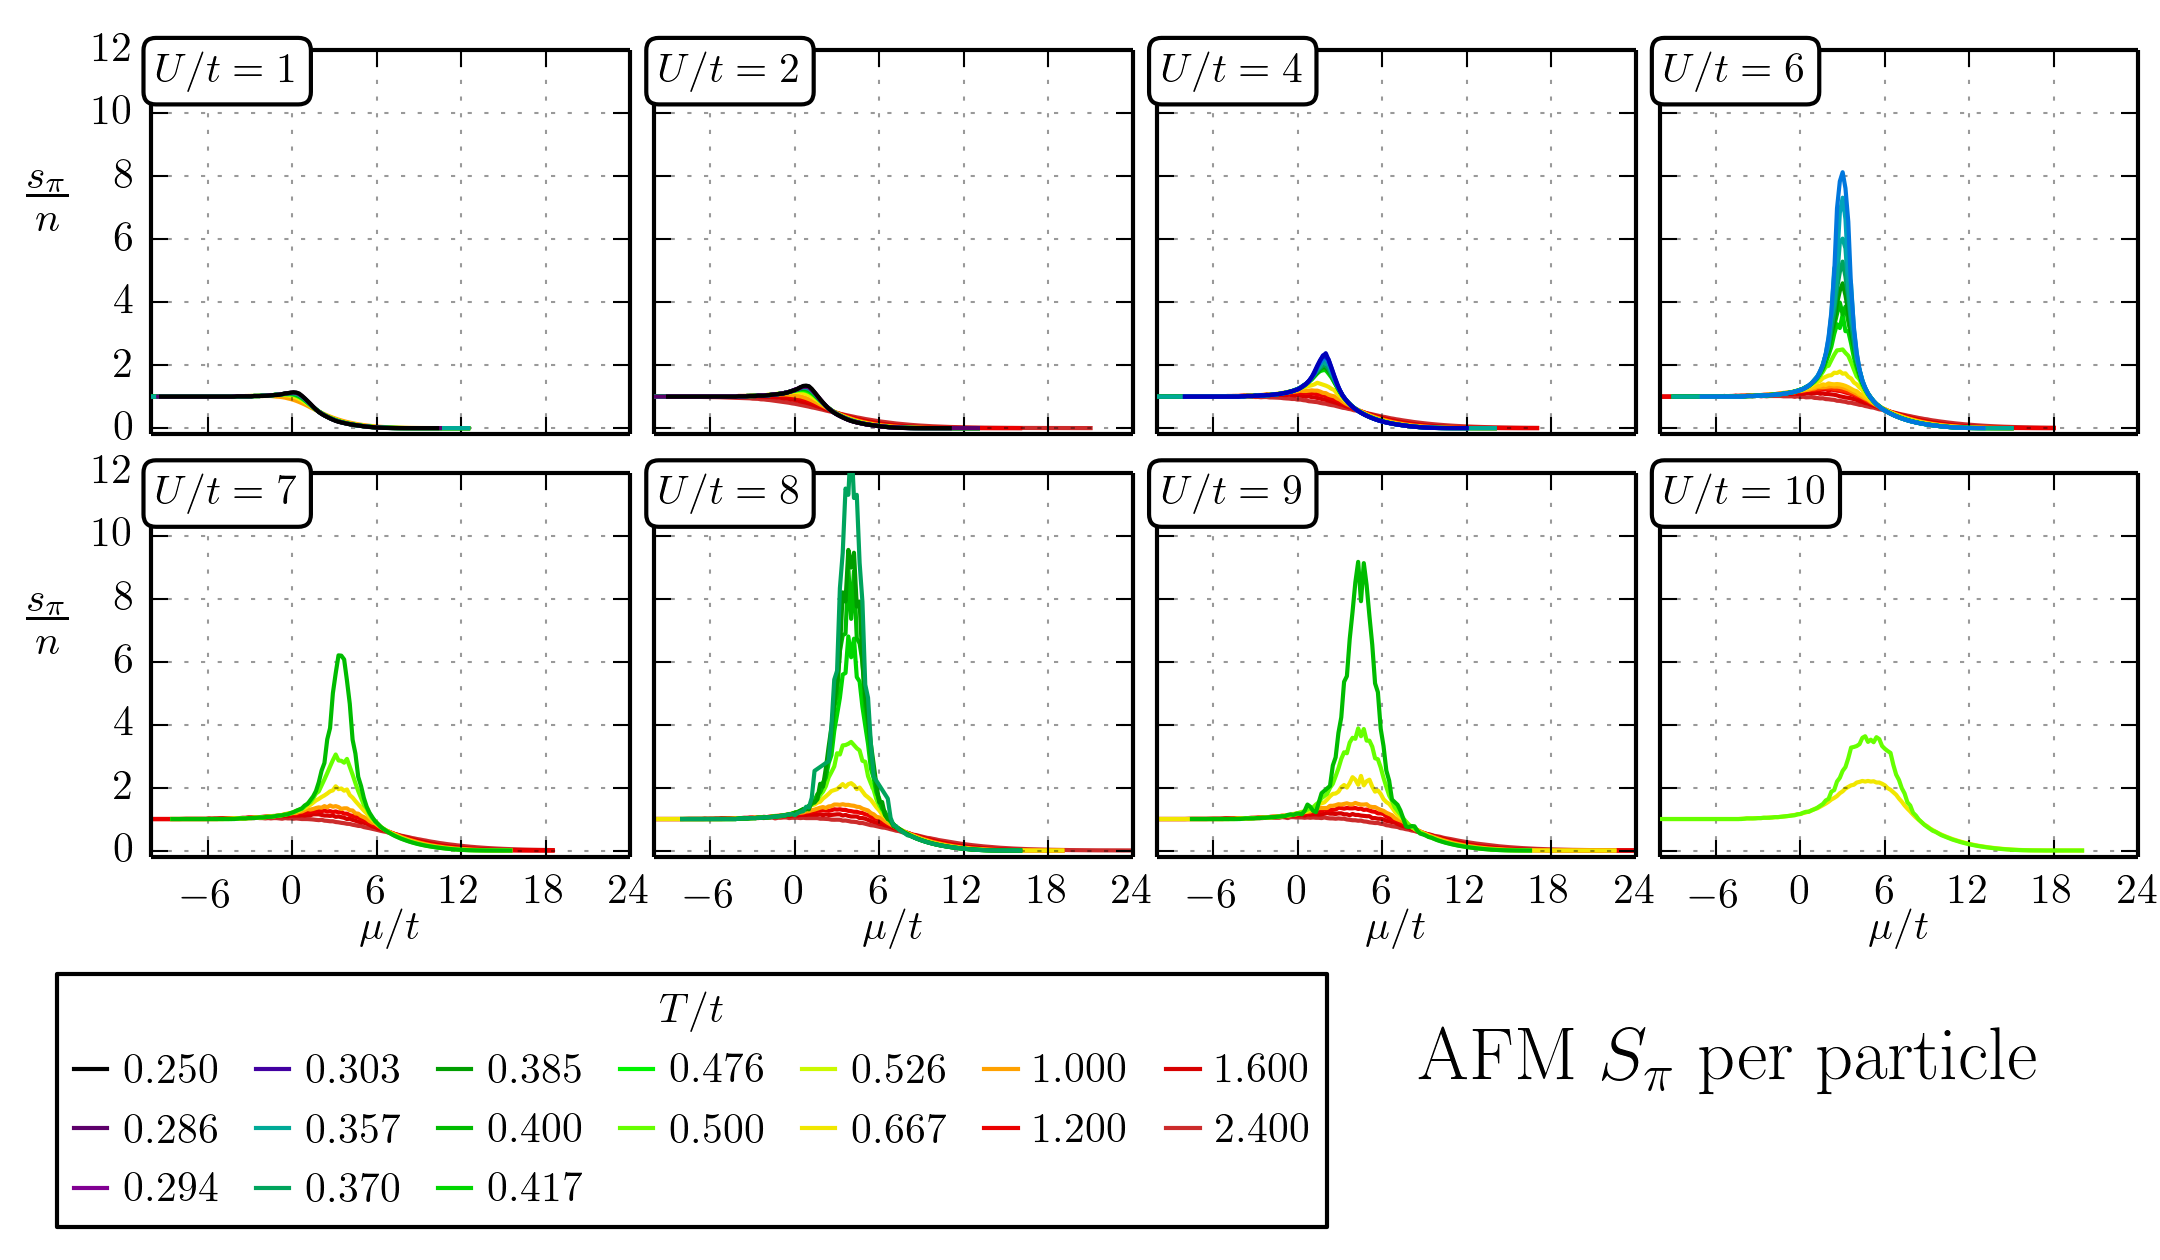
\includegraphics[width=1.0\textwidth]{../figures/hubbard-data/dataplots/QMC_Final/spi_n_10.png}
\caption{ DQMC results for the spin structure factor per particle at
$\bv{Q}=\bv{\pi}$. } 
\label{fig:QMCspi}
\end{figure}
\begin{figure}
    \centering
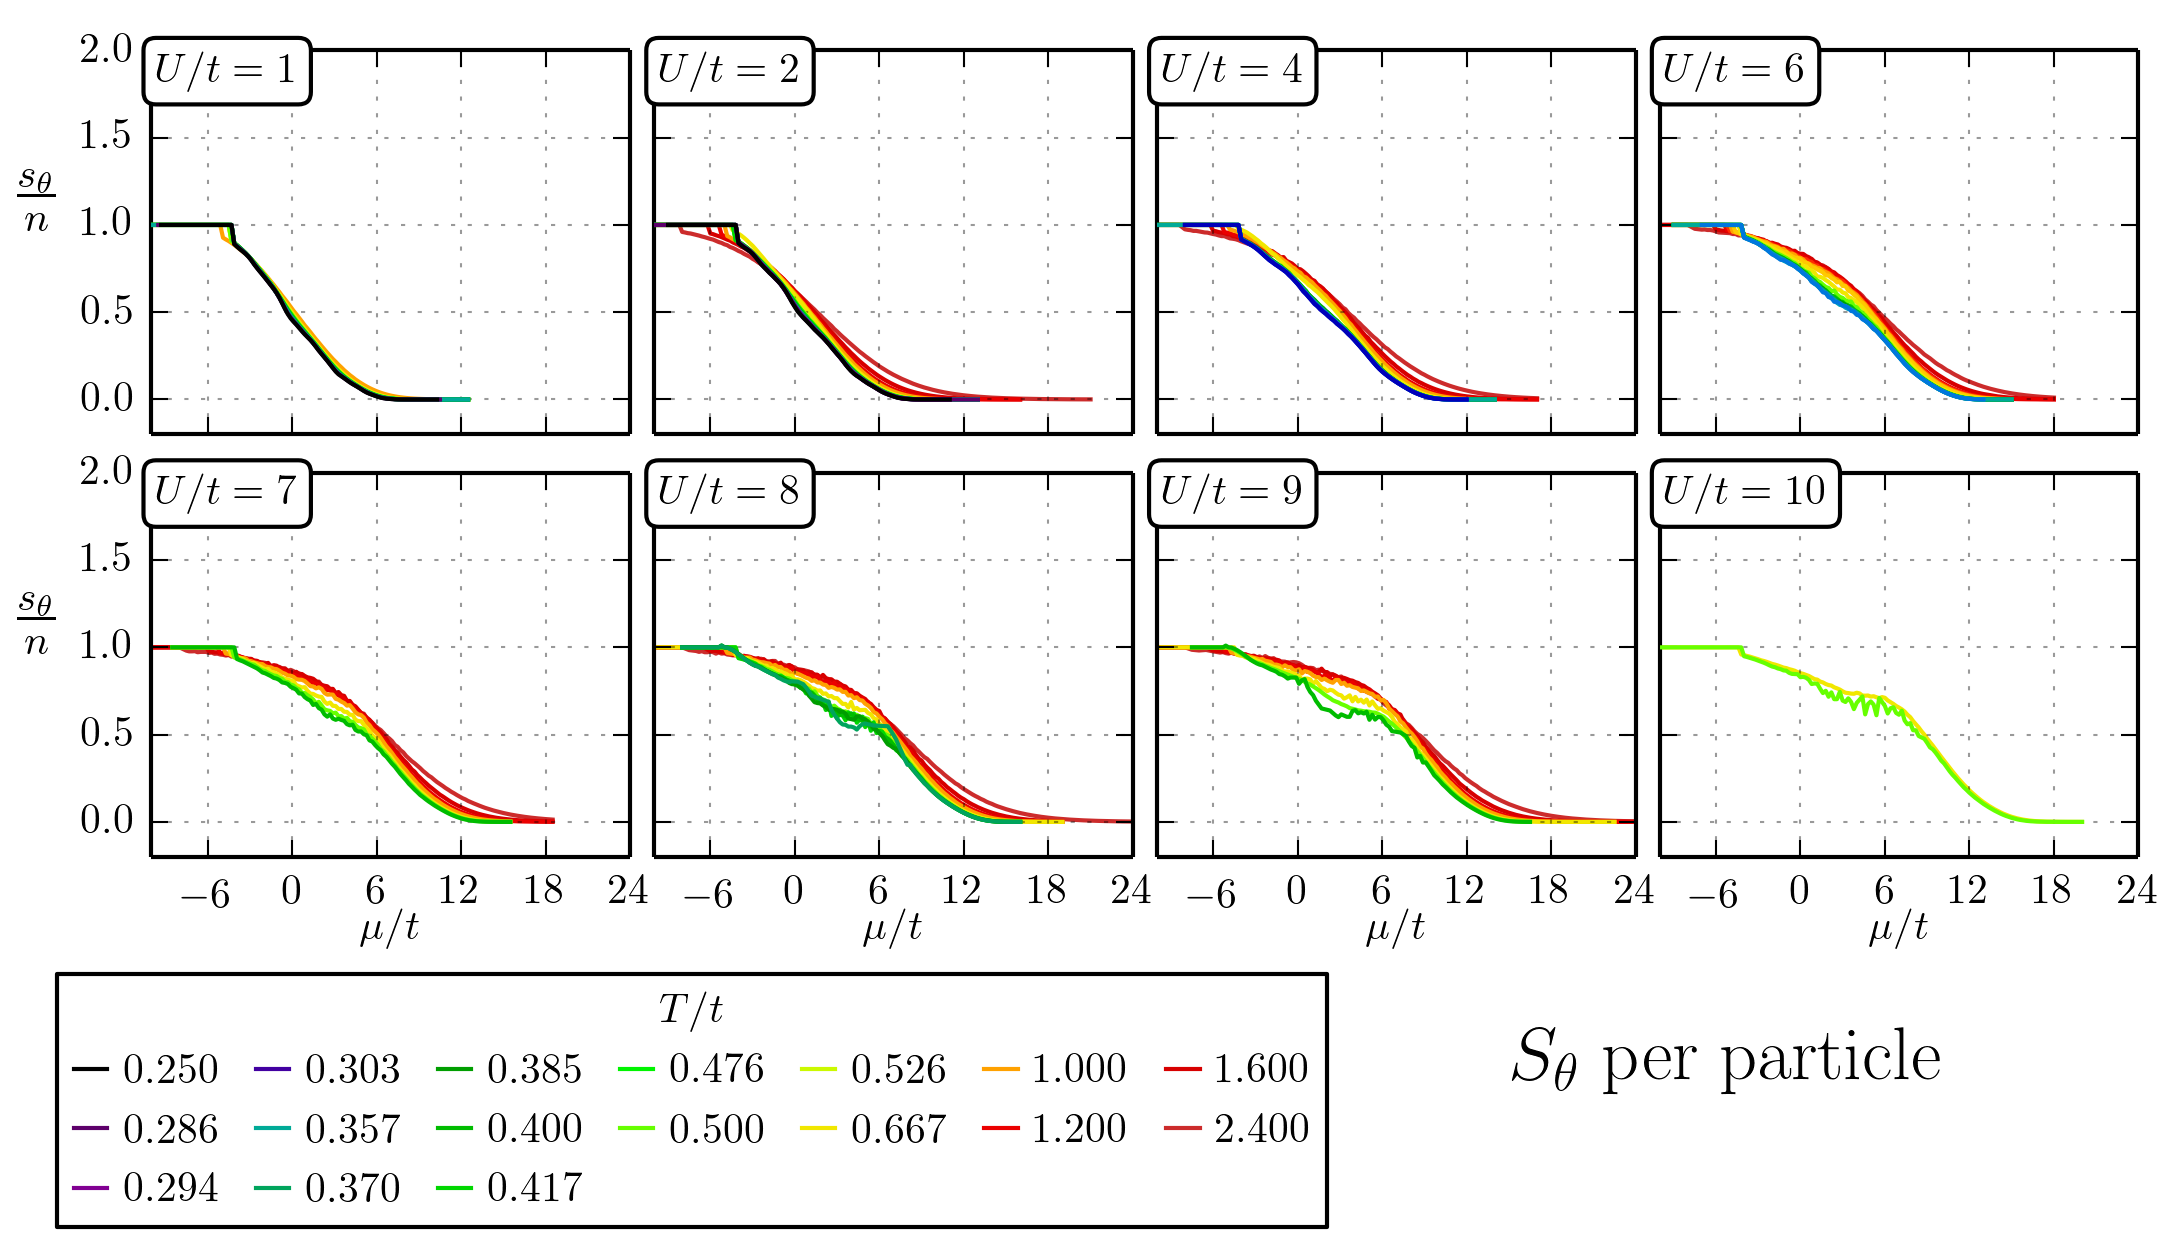
\includegraphics[width=1.0\textwidth]{../figures/hubbard-data/dataplots/QMC_Final/sth_n_10.png}
\caption{ DQMC results for the spin structure factor per particle at
$\bv{Q}=\bv{\theta}$. } 
\label{fig:QMCsth}
\end{figure}
 


\section{ DQMC and NLCE comparison} 

In Fig.~\ref{fig:QMCvsNLCE} we show DQMC and NLCE results for density and
$s_{\bv{\pi}}$ for $U/t=6$ and $U/t=8$.  It is clear from this plot that the
density is ``frozen'' for $T/t < 1.0$ and that both QMC and NLCE have very good
agreement on the density.   We also see that NLCE overestimates $s_{\bv{\pi}}$
slightly with respect to DQMC. 
\begin{figure}
    \centering
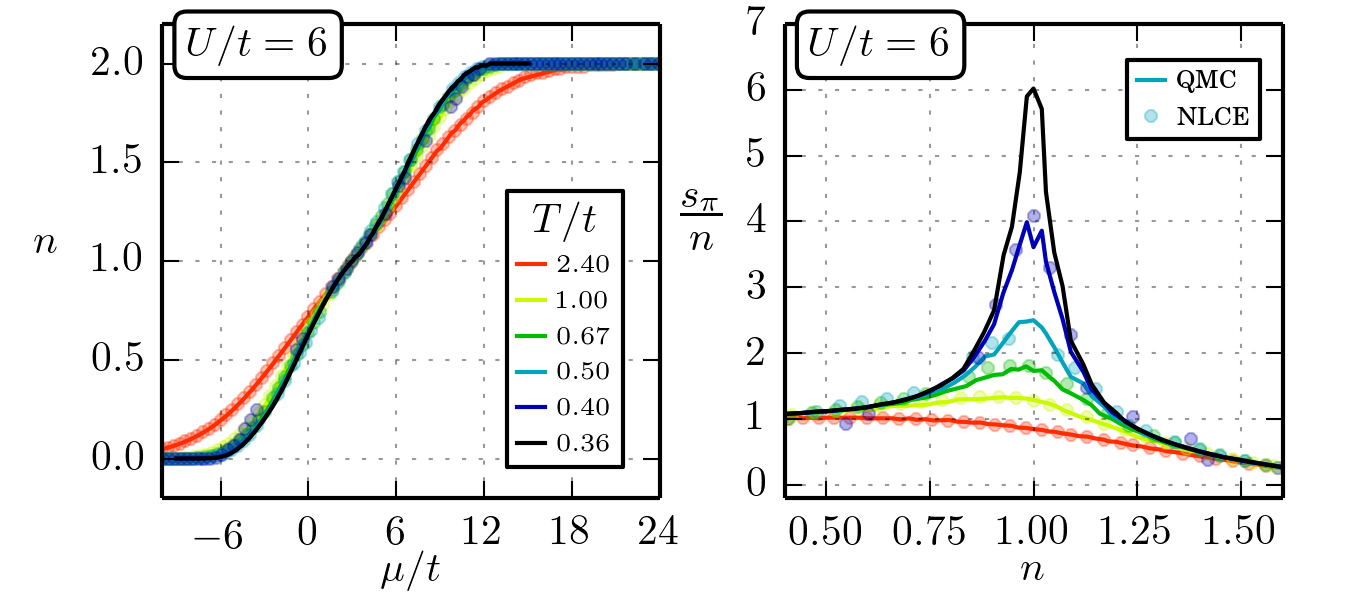
\includegraphics[width=\textwidth]{../figures/hubbard-data/dataplots/QMC_Final/QMC_NLCE_Compare_U06.png}
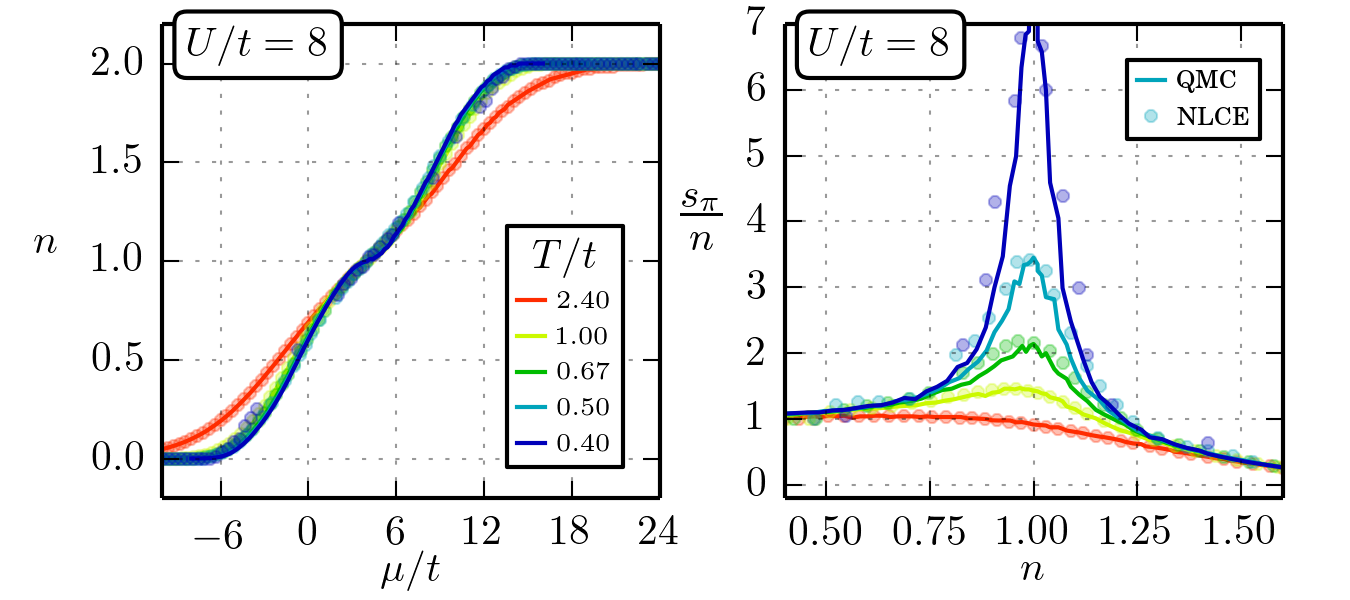
\includegraphics[width=\textwidth]{../figures/hubbard-data/dataplots/QMC_Final/QMC_NLCE_Compare_U08.png}
\caption{Comparison between DQMC and NLCE data.  DQMC result are shown as lines
and NLCE result are shown as points.  } \label{fig:QMCvsNLCE}
\end{figure}

%\section{ Spin structure factor }
%
%Our experiment measures the bulk spin structure factor $\bar{S}_{\bv{Q}}$ for
%an inhomogeneous realization of the Hubbard model.  Theoretical approaches such
%as QMC and NLCE consider a homogeneous system with a finite number of lattice
%sites $L^{3}$ and  calculate the structure factor 
%\begin{equation} 
%    S_{\bv{Q}} = \frac{4}{L^{3}} \sum_{i,j} 
%     e^{i\bv{Q}\cdot ( \bv{R}_{i} - \bv{R}_{j} )} \langle \sigma_{zi} \sigma_{zj}  \rangle
%\end{equation}
%
%In the local density approximation we can think of every point $\bv{r}$ of our
%lattice site as a homogeneous system for which $S_{\bv{Q}}(\bv{r})$ can be
%obtained.  We can relate the measured bulk spin structure factor
% to the local $S_{\bv{Q}}(\bv{r})$ as
%\begin{equation}
%  \bar{S}_{\bv{Q}}  = \frac{1}{N} \int  S_{\bv{Q}}(\bv{r}) \, \mathrm{d}^{3} \bv{r}
%\end{equation}
%
%The NLCE data provided by Ehsan gives $S_{\bv{Q}}$ directly whereas the QMC
%data provided by Thereza gives $S_{\bv{Q}}/n$.  To compare with experiment we
%have decided to use $S_{\bv{Q}}/n$ such that  
%\begin{equation}
%  \bar{S}_{\bv{Q}}  = \frac{1}{N} 
%   \int \left[ \frac{  S_{\bv{Q}} }{n} \right]_{\bv{r}}
%    n(\bv{r})  \, \mathrm{d}^{3} \bv{r}
%\end{equation}
%
%Also, in our LDA calculations we have assumed that there is spherical symmetry
%in the system so 
%\begin{equation}
%  \bar{S}_{\bv{Q}}  = \frac{4\pi}{N} 
%   \int \left[ \frac{  S_{\bv{Q}} }{n} \right]_{r_{d}}
%    n(r_{d}) \,\, r_{d}^{2}   \, \mathrm{d}r_{d}
%\end{equation}
%where $r_{d}$ is the distance from the origin along a 111 body diagonal of the
%lattice.  
%
%The validity of the spherical symmetry assumption is very questionable, since
%away from the diagonal the lattice depths are different along the $x,y,z$
%directions and an anisotropic Hubbard model should be used. However, for
%simplicity this is how we decided to treat the system.

\section{ Implementation of the local density approximation } 

We implement the LDA according to the following steps: 
\begin{enumerate}

  \item Set up a trap geometry based on our experimental calibration of the
lattice beam waists.  Even though the beam waists differ slightly for the three
axis, we model the system with a potential that has full cubic symmetry.
Furthermore, we assume that the sample is spherically symmetric and only
calculate thermodynamic quantities along a body diagonal of the lattice. In the
experiment we adjust the values of the compensation along each axes to aim for
production of nearly spherically symmetric samples. 

 \item  Set the temperature $T$, and the global chemical potential $\mu_{0}$.
The trap geometry, along with $\mu_{0}$, then determines the local $\mu/t$, the
local $U/t$ and the local $T/t$. 

  \item Perform a calculation of the local density and integrate it to find the atom number, $N$, in the trap. 

  \item Repeat steps 2 and 3 until the value of $\mu_{0}$ is found that
produces the atom number desired for the simulation. 

  \item Once the value of $\mu_{0}$ is found, go ahead and calculate profiles
and bulk values for other thermodynamic quantities (entropy, $s_{\bv{\pi}}$,
and $s_{\bv{\theta}}$).

\end{enumerate}

\subsection{ Determination of thermodynamic quantities by interpolation between
available data}

Any local thermodynamic quantity $q(r)$ depends on the local values of the
Hubbard parameters: $\mu/t$, $U/t$ and $T/t$.  As we move along the body
diagonal of the lattice calculating values of $q(r)$, we will encounter
particular values of the Hubbard parameters that are not part of the data set
of DQMC and NLCE numerical results.   For arbitrary values of the Hubbard
parameters we carry out a linear interpolation in the following way:

\begin{figure}
    \centering
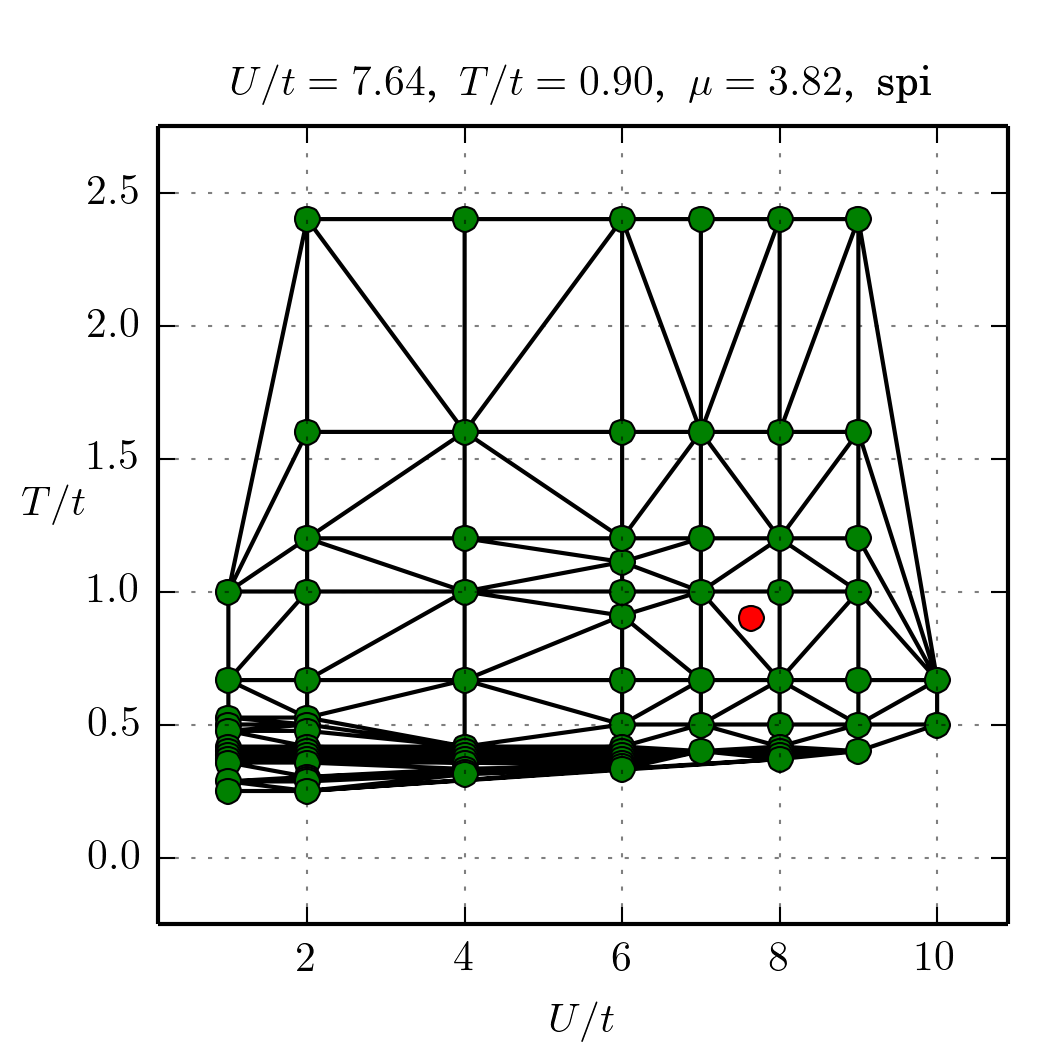
\includegraphics[width=0.5\textwidth]{../figures/hubbard-data/dataplots/interp/qmcpts_141013.png}
\caption{Delaunay triangulation for the full grid of $U/t$ and $T/t$ values
provided by the DQMC data set.  In this example we are interested in
calculating $s_{\bv{\pi}}$ at values of the Hubbard parameters $U/t=7.64$ and
$T/t=0.9$. }
\label{fig:delaunay-example}
\end{figure}

\begin{enumerate}

 \item  We create a Delaunay triangulation of the available $U/t$ and $T/t$
data points that are closest to the Hubbard parameters of interest.  An example of this triangulation is shown in Fig.~\ref{fig:delaunay-example}. 

 \item  The triangulation defines three ($U/t,T/t$) points that surround the
point of interest.  For each of these three points, we look into the available
data and find the value of the thermodynamic quantity $q(\mu/t)$ for the
chemical potential of interest.  For this look-up we linearly interpolate
between the available values of the chemical potential in the data set. 

 \item  At this point we have the values of $q$ at the three vertices of the
triangle that surrounds the ($U/t,T/t$) point of interest.  These three
vertices define a plane in  ($U/t,T/t,q$)-space which we use to linearly
interpolate and find the value of $q$ that we are looking for. 
\end{enumerate}

In Fig.~\ref{fig:delaunay-all} we shown all of the combined DQMC and NLCE
points in the $U/t,T/t$ grid that is used for interpolation. 

\begin{figure}
    \centering
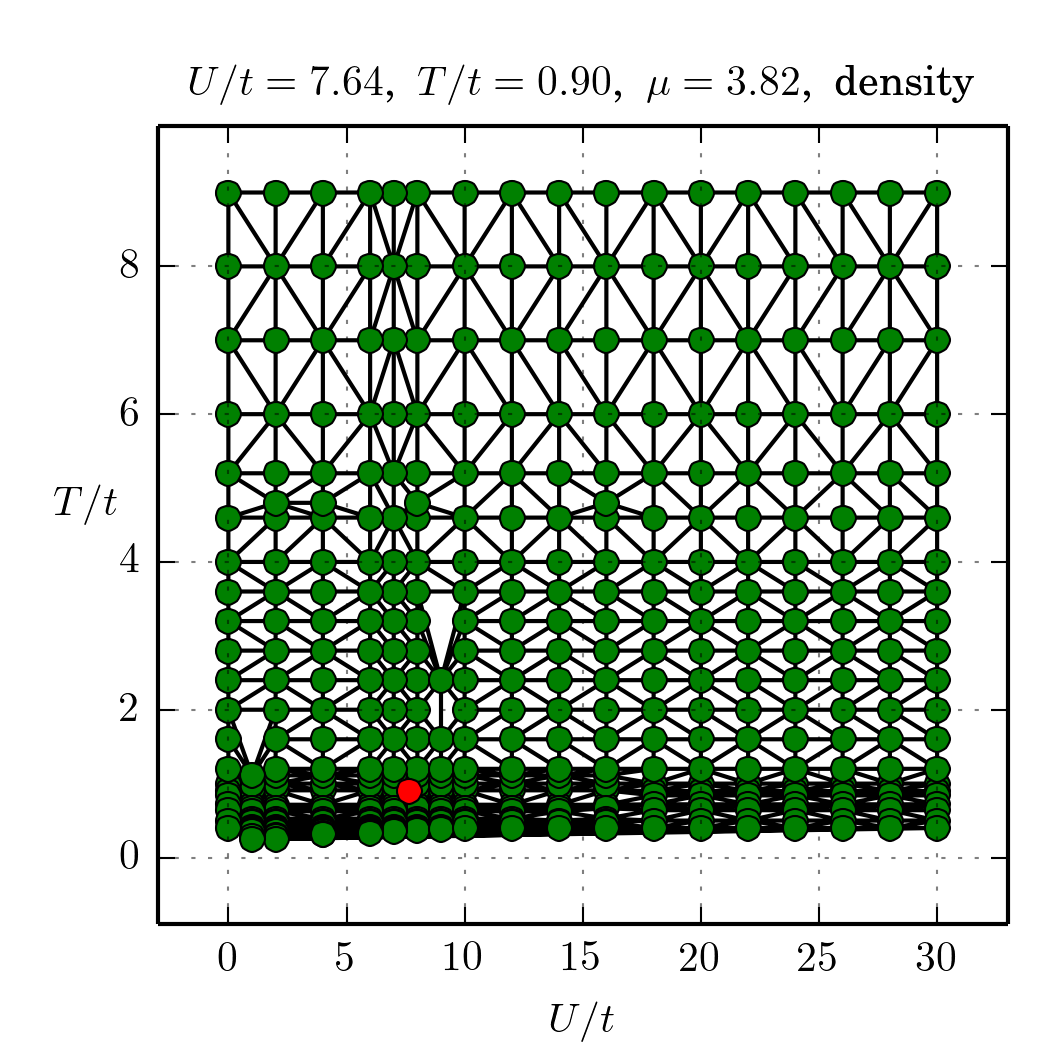
\includegraphics[width=0.75\textwidth]{../figures/hubbard-data/dataplots/interp/allpts_141014.png}
\caption{All of the available ($U/t,T/t$) data points in the combined DQMC and
NLCE data sets for the density. The red point is the same as in the example
shown in Fig.~\ref{fig:delaunay-example}. }
\label{fig:delaunay-all}
\end{figure}
 




